\documentclass[11pt]{article}
\usepackage[review]{acl}
\usepackage{times}
\usepackage{multirow}
\usepackage{latexsym}
\usepackage[T1]{fontenc}
\usepackage[utf8]{inputenc}
\usepackage{microtype}
\usepackage{inconsolata}
\usepackage{amsmath}
\usepackage{amssymb}
\usepackage{booktabs}
\usepackage{enumitem}
\usepackage{graphicx}
\usepackage{listings}
\usepackage{tikz}
\usepackage{xcolor}

\lstset{
  basicstyle=\ttfamily\scriptsize,
  breaklines=true,
  breakatwhitespace=false,
  frame=single,
  framesep=2pt,
  columns=fullflexible,
  keepspaces=true,
  xleftmargin=2pt,
  xrightmargin=2pt,
  aboveskip=4pt,
  belowskip=4pt,
  escapeinside={(*@}{@*)},
}


\usetikzlibrary{positioning, arrows.meta, fit, backgrounds, shapes.geometric, calc}


\title{AILS-NTUA at SemEval-2026 Task 10:}


\author{First Author \\
  Affiliation / Address line 1 \\
  Affiliation / Address line 2 \\
  Affiliation / Address line 3 \\
  \texttt{email@domain} \\\And
  Second Author \\
  Affiliation / Address line 1 \\
  Affiliation / Address line 2 \\
  Affiliation / Address line 3 \\
  \texttt{email@domain} \\}

\begin{document}
\maketitle
\begin{abstract}
    This document is a supplement to the general instructions for *ACL authors. It contains instructions for using the \LaTeX{} style files for ACL conferences.
    The document itself conforms to its own specifications, and is therefore an example of what your manuscript should look like.
    These instructions should be used both for papers submitted for review and for final versions of accepted papers.
\end{abstract}

\section{Introduction}
Humans have long exhibited a tendency to endorse conspiracy theories,
particularly in contexts of uncertainty, threat, and social upheaval. Such
beliefs are created and distributed to support human need for addressing
existential or social issues and strengthen their sense of identity and
belonging \cite{psychology-of-conspiracy, belief}. Despite their psychological
appeal, conspiracies are associated with harmful consequences, limiting trust
in well-documented facts and public decisions, while exacerbating political
polarization and misinformation patterns \cite{understanding}.

The rise of artificial intelligence inspired the connection of conspiracy
identification with natural language, as language constitutes the most
fundamental medium for conspiracy articulation and spread. Conspiratorial
statements are subtly embedded in language exploiting linguistic strategies to
evoke emotions and attribution of agency \cite{miani2022loco,
    rains2023psycholinguistic}, suggesting that conspiracy identification goes well
beyond superficial linguistic cues.

Large Language Models (LLMs) have revolutionized linguistic research, enabling
deep pattern identification and discrimination among their numerous abilities.
However, LLMs have been found to be significantly prone to cognitive biases
\cite{filandrianos-etal-2025-bias} and manipulation via persuasive language
\cite{xu-etal-2024-earth}, while they generate and amplify misinformation
\cite{chen2024combatingmisinformation}. Going one step further,
state-of-the-art LLMs are even able to persuade people to adopt conspiratorial
beliefs to a comparable degree as they can mitigate conspiracy dissemination
\cite{costello2026largelanguagemodelseffectively}, exposing the double-edged
nature of LLMs in the context of factual verification.

The core challenges that conspiratorial discourse poses call for fine-grained
data approaches that allow delving into the linguistic mechanisms that
characterize conspiratorial utterances in an interpretable way. Nevertheless,
prior datasets \cite{shahsavari2020conspiracy, langguth2023coco} frame
conspiracy detection as a coarse-grained classification task, abstracting away
from the particularities of conspiratorial discourse, thus obscuring how
conspiratorial reasoning is formed and expressed in language. To fill this gap,
the \textbf{SemEval 2026 Task 10: Psycholinguistic Conspiracy Marker Extraction
    and Detection} emphasizes the localization and categorization of linguistic
markers that signal conspiratorial thinking, complementing detection with
psychologically-backed annotations.

To address the dual challenges of accurate detection and interpretable marker
extraction, models must be capable of capturing both global conspiratorial
intent and fine-grained psycholinguistic cues embedded in language. In our
approach, we leverage LLMs within agentic structures to advance the recognition
of conspiratorial thought. Specifically, [] To the best of our knowledge, we
introduce the \textit{first agentic LLM-based method} to combat conspiracy
detection and identification of psycholinguistic features in language.

In short, our contributions are the following:
\begin{itemize}
    \item We introduce the first agentic LLM-based method for psycholinguistic conspiracy
          marker extraction and detection.
\end{itemize}

\section{Background}
\paragraph{Task description}
The dataset comprises 4,800 annotations spanning 4,100 unique Reddit submission
statements from $>$190 subreddits, divided in two subtasks: \textbf{\textit{i)}
    S1: Conspiracy Marker Extraction} contains textual spans that express core
conspiracy markers grounded in evolutionary psychology. One or more marker
types may appear in each comment, falling in the following categories:
\textsc{Actor} (mentions of individual or group agents), \textsc{Action}
(descriptions of what the actor is doing), \textsc{Effect} (consequences of the
actions), \textsc{Victim} (who is being harmed), \textsc{Evidence} (claims or
proof used to support the theory). \textbf{\textit{ii)} S2: Conspiracy
    Detection} assigns conspiracy-related or not conspiracy-related labels to
Reddit comments. More details about the dataset are provided in App.
\ref{sec:eda}.

\paragraph{Related work} Early works on NLP conspiratorial discourse on Reddit introduced narrative
motifs correlated with conspiratorial evidence \cite{online-discussions} and
demonstrated that conspiratorial thinking manifests through detectable
psycholinguistic signals in user language \cite{Klein2019Pathways}, with
consequent literature revealing that conspiracy theories exhibit distinctive
narrative frameworks that can be computationally extracted from text
\cite{Tangherlini2020Automated}. These foundational works empowered the
operationalization of conspiracy identification as a classification task,
exemplified by datasets such as COCO \cite{langguth2023coco} and YouNICon
\cite{YouNICon}. Conspiracy detection involves techniques that explicitly model
psycholinguistic signals, such as affective tone, attributional cues and
explanatory framing, in order to provide explanatory evidence of conspiracy
presence in language \cite{rains2023psycholinguistic,
    language-of-conspiracy-theories, marino-etal-2025-linguistic}. The strong
contextualization that LLMs offer inspired the introduction of related
approaches; leveraging appropriate prompting enables accurate multi-label
conspiracy classification, eliminating training demands
\cite{peskine-etal-2023-definitions}. Complementarily, ConspEmoLLM
\cite{liu2024conspemollm} involves emotion-aware LLM fine-tuning on several
conspiratorial tasks, improving detection by leveraging affective signals, with
subsequent extensions focusing on robustness to stylistic and emotional
variation \cite{liu2025conspemollmv2}. Recent evaluations indicate that
LLM-based conspiracy detection often relies on topical shortcuts and struggles
with narrative ambiguity, underscoring the need for approaches grounded in
interpretable psycholinguistic markers \cite{pustet-etal-2024-detection,
    classifying}.

\section{System Overview}

We present an \textbf{agentic LLM architecture} that decomposes the dual
challenges of marker extraction and conspiracy detection into specialized,
interacting agents orchestrated via stateful workflows. Unlike monolithic
prompting approaches that conflate reasoning steps within a single LLM call,
our system explicitly separates \textit{generation}, \textit{critique},
\textit{refinement}, and \textit{verification} into distinct computational
nodes with typed interfaces. An overview of the system is illustrated in Figure
\ref{fig:arch}.

\begin{figure*}[t]
    \centering
    \small
    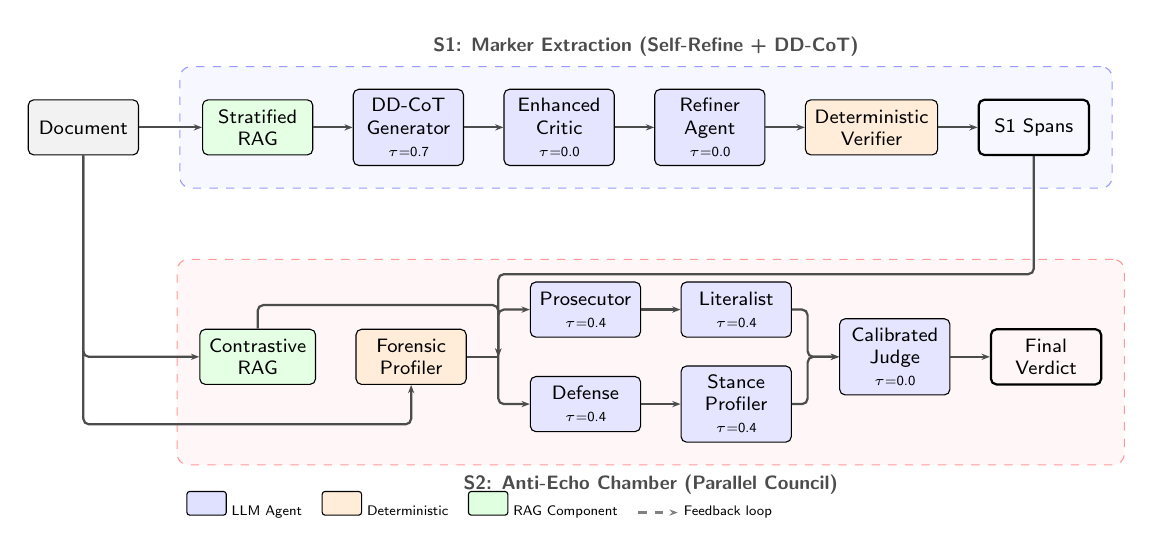
\begin{tikzpicture}[
        node distance=0.6cm and 0.4cm,
        >={Stealth[length=3pt]},
        % Styles
        inputbox/.style={rectangle, draw, rounded corners=2pt, minimum height=0.7cm,
                minimum width=1.4cm, align=center, font=\scriptsize\sffamily, fill=gray!10},
        ragbox/.style={rectangle, draw, rounded corners=2pt, minimum height=0.7cm,
                minimum width=1.4cm, align=center, font=\scriptsize\sffamily, fill=green!10},
        llmbox/.style={rectangle, draw, rounded corners=2pt, minimum height=0.7cm,
                minimum width=1.4cm, align=center, font=\scriptsize\sffamily, fill=blue!10},
        detbox/.style={rectangle, draw, rounded corners=2pt, minimum height=0.7cm,
                minimum width=1.4cm, align=center, font=\scriptsize\sffamily, fill=orange!15},
        outputbox/.style={rectangle, draw, rounded corners=2pt, minimum height=0.7cm,
                minimum width=1.4cm, align=center, font=\scriptsize\sffamily, thick},
        arrow/.style={->, thick, black!70, rounded corners=2pt}, dasharrow/.style={->,
                thick, dashed, black!50, rounded corners=2pt},
        grouplab/.style={font=\bfseries\scriptsize\sffamily, text=black!70},
        labeltext/.style={font=\tiny\sffamily, text=black!60, midway, fill=white, inner
                sep=1pt}, ]

        % === INPUT ===
        \node[inputbox] (input) {Document};

        % === S1 PIPELINE (Top Row) ===
        \node[ragbox, right=0.8cm of input] (s1rag) {Stratified\\RAG};
        \node[llmbox, right=0.5cm of s1rag] (gen) {DD-CoT\\Generator\\{\tiny $\tau$=0.7}};
        \node[llmbox, right=0.5cm of gen] (critic) {Enhanced\\Critic\\{\tiny $\tau$=0.0}};
        \node[llmbox, right=0.5cm of critic] (refiner) {Refiner\\Agent\\{\tiny $\tau$=0.0}};
        \node[detbox, right=0.5cm of refiner] (verifier) {Deterministic\\Verifier};
        \node[outputbox, right=0.5cm of verifier] (s1out) {S1 Spans};

        % S1 Connections
        \draw[arrow] (input) -- (s1rag);
        \draw[arrow] (s1rag) -- (gen);
        \draw[arrow] (gen) -- (critic);
        \draw[arrow] (critic) -- (refiner);
        \draw[arrow] (refiner) -- (verifier);
        \draw[arrow] (verifier) -- (s1out);

        % S1 Group Label
        \begin{scope}[on background layer]
            \node[draw=blue!40, fill=blue!3, rounded corners=4pt, dashed,
            fit=(s1rag)(gen)(critic)(refiner)(verifier)(s1out),
            inner sep=8pt, label={[grouplab]above:{S1: Marker Extraction (Self-Refine + DD-CoT)}}] (s1group) {};
        \end{scope}

        % === S2 PIPELINE (Bottom Row) ===
        \node[ragbox, below=2.2cm of s1rag] (s2rag) {Contrastive\\RAG};
        \node[detbox, right=0.5cm of s2rag] (forensic) {Forensic\\Profiler};

        % PARALLEL COUNCIL (Strict 2x2 Grid)
        \node[llmbox, right=0.8cm of forensic, yshift=0.6cm] (pros) {Prosecutor\\{\tiny $\tau$=0.4}};
        \node[llmbox, right=0.5cm of pros] (literal) {Literalist\\{\tiny $\tau$=0.4}};

        \node[llmbox, right=0.8cm of forensic, yshift=-0.6cm] (defense) {Defense\\{\tiny $\tau$=0.4}};
        \node[llmbox, right=0.5cm of defense] (profiler) {Stance\\Profiler\\{\tiny $\tau$=0.4}};

        % Judge
        \node[llmbox, right=0.6cm of $(literal.east)!0.5!(profiler.east)$] (judge) {Calibrated\\Judge\\{\tiny $\tau$=0.0}};
        \node[outputbox, right=0.5cm of judge] (verdict) {Final\\Verdict};

        % Fork (Clean Distribution)
        \coordinate[right=0.4cm of forensic] (fork_point);
        \draw[thick, black!70] (forensic.east) -- (fork_point);
        \draw[arrow] (fork_point) |- (pros.west);
        \draw[arrow] (fork_point) |- (defense.west);

        % S2 Connections
        \draw[arrow] (input.south) |- (s2rag.west);
        \draw[arrow] (input.south) |- ($(s2rag.south) + (0,-0.5)$) -| (forensic.south);

        % S1 Out to Council 
        \draw[arrow] (s1out.south) -- ++(0,-1.5) -| (fork_point);

        % S2RAG to Council (Bypassing Forensic)
        \draw[arrow] (s2rag.north) -- ++(0,0.3) -| (fork_point);

        % Internal Flow
        \draw[arrow] (pros) -- (literal);
        \draw[arrow] (defense) -- (profiler);

        % Merge (Clean Join)
        \draw[arrow] (literal.east) -- ++(0.2,0) |- (judge.west);
        \draw[arrow] (profiler.east) -- ++(0.2,0) |- (judge.west);
        \draw[arrow] (judge) -- (verdict);

        % S2 Group Label
        \begin{scope}[on background layer]
            \node[draw=red!40, fill=red!3, rounded corners=4pt, dashed,
            fit=(s2rag)(forensic)(pros)(defense)(literal)(profiler)(judge)(verdict),
            inner sep=8pt, label={[grouplab]below:{S2: Anti-Echo Chamber (Parallel Council)}}] (s2group) {};
        \end{scope}

        % Legend
        \node[below=0.2cm of s2group.south west, anchor=north west, font=\tiny\sffamily] (leg) {
            \tikz\node[fill=blue!12, draw, rounded corners=1pt, minimum height=0.3cm, minimum width=0.5cm] {}; LLM Agent \quad
            \tikz\node[fill=orange!15, draw, rounded corners=1pt, minimum height=0.3cm, minimum width=0.5cm] {}; Deterministic \quad
            \tikz\node[fill=green!12, draw, rounded corners=1pt, minimum height=0.3cm, minimum width=0.5cm] {}; RAG Component \quad
            \tikz\draw[->, thick, dashed, black!50] (0,0) -- (0.5,0); Feedback loop
        };

    \end{tikzpicture}
    \caption{System architecture overview. \textbf{S1} (top): The DD-CoT Self-Refine pipeline extracts markers via Generate $\rightarrow$ Critique $\rightarrow$ Refine. \textbf{S2} (bottom): The Anti-Echo Chamber classifies conspiracy stance. All prompts were optimized via GEPA. Temperature settings ($\tau$) are role-specific: high exploration for the Generator ($\tau=0.7$), balanced debate for the Parallel Council ($\tau=0.4$), and deterministic evaluation for Critics and Judges ($\tau=0.0$).}
    \label{fig:arch}
\end{figure*}

\subsection{S1: Marker Extraction via DD-CoT}

We formulate marker extraction as a \textbf{hybrid extraction strategy} that
separates semantic reasoning from structural localization, implemented through
a four-node graph that contains: document text, few-shot examples, text
complexity assessment, dominant narrative type, draft extractions, critic
feedback, and final verified spans. %LangGraph 

\paragraph{Hybrid Architecture Rationale.} A critical design decision is the explicit separation of \textit{semantic
    identification} from \textit{span indexing}. LLMs excel at understanding
\textit{what} constitutes a psycholinguistic marker and \textit{why} it belongs
to a particular category, but they are inherently unreliable at character-level
token counting \cite{fu2024struggle}. Consequently, we employ a two-stage strategy: (i) the LLM
serves as a \textbf{semantic reasoner}, identifying marker text strings and
their labels through reasoning chains; (ii) a deterministic Python-based
\textbf{structural locator} performs exact string matching to compute character
offsets (\texttt{startIndex}, \texttt{endIndex}). This hybrid approach
eliminates the ``hallucinated span'' problem, i.e. instances where the LLM
correctly identifies marker semantics but produces invalid or off-by-one
character indices \cite{ogasa-arase-2025-hallucinated}.%---a well-documented limitation in autoregressive transformers that lack explicit positional grounding during generation

\paragraph{Dynamic Discriminative Chain-of-Thought (DD-CoT).} Our core methodological contribution extends standard chain-of-thought (CoT)
reasoning \cite{wei2022chain} by requiring the model to articulate both
inclusion \textit{and} exclusion criteria for each candidate span. For each
extracted marker, the LLM must justify the following: (i) \textit{Why
    \textbf{this} label}: evidence supporting the assigned category (e.g.,
``extracted as \textsc{Actor} because it names a collective agent with alleged
malicious intent''); and (ii) \textit{Why \textbf{not} other labels}: explicit
discrimination against confusable alternatives (e.g., ``not \textsc{Victim}
because this entity performs the action rather than receiving harm''). This
discriminative reasoning directly addresses the primary source of error
identified in our early development: label confusion between semantically
adjacent categories such as \textsc{Actor}$\leftrightarrow$\textsc{Victim} and
\textsc{Action}$\leftrightarrow$\textsc{Effect}.%generator 

\paragraph{Agents} comprise the following graph nodes:
\begin{enumerate}
    \item \textbf{DD-CoT Generator:} Produces candidate spans with discriminative rationales using DD-CoT, text complexity assessment (simple, moderate, complex), and dominant narrative classification (accusatory, victimhood, exposure) at temperature $\tau=0.7$ for exploration. Crucially, the LLM outputs only the marker text string and label, and refrains from generating character indices at this stage.
    \item \textbf{Enhanced Critic:} Audits extractions from DD-CoT Generator for verbatim accuracy, granularity violations (single-word spans, full-sentence spans), label consistency, and exhaustiveness (missed markers). It implements a \textit{Soft Gate} mechanism that intercepts overly aggressive ``remove all'' directives when the draft contains structurally significant extractions (\textsc{Actor}--\textsc{Action} pairs), forcing granular refinement instead of total wipes.

    \item \textbf{Refiner:} Applies targeted corrections based on the Critic's feedback while preserving valid spans, operating purely on text strings without index manipulation. %It receives narrative and complexity context to enable appropriate boundary expansion for complex texts  

    \item \textbf{Deterministic Verifier:} A non-LLM post-processing node that serves as the \textit{structural locator}, anchoring LLM-generated text strings to character-precise offsets through a five-tier matching cascade:
          \begin{enumerate}
              \item[(i)] \textbf{Exact match:} Byte-for-byte substring search supporting nth-occurrence disambiguation.
              \item[(ii)] \textbf{Case-insensitive:} Unicode-safe lowered comparison with original-position projection.
              \item[(iii)] \textbf{Normalized:} Smart-quote straightening, whitespace collapse, and lowering with index remapping to recover original character offsets.
              \item[(iv)] \textbf{Fuzzy (Levenshtein):} Approximate matching with maximum edit distance $\leq 15\%$ of snippet length (minimum~1), activated only for spans $>$4 characters to avoid spurious short matches.
              \item[(v)] \textbf{SequenceMatcher alignment:} LCS-based last-resort recovery requiring $\geq 60\%$ character coverage and compactness $\leq 1.5\times$ snippet length, with word-boundary snapping.
          \end{enumerate}
          Each tier is attempted in order; the first successful match is accepted. Additionally, the Verifier implements aggressive cross-label deduplication to eliminate overlapping or duplicate spans. This graduated recovery strategy ensures that all submitted spans are structurally valid and anchored to the source text, even when upstream LLM paraphrases or reformulations introduce minor textual divergence from the original document.
\end{enumerate}

\paragraph{Self-Refine}  provides feedback on an LLM's own outputs and refines consequent generation
\cite{madaan2023selfrefine}, operating on the agentic graph by executing the
four nodes sequentially.

\subsection{S2: Classification via Anti-Echo Chamber}

The principal challenge in conspiracy detection is distinguishing \textit{topic
    presence} from \textit{stance endorsement}, a phenomenon we term the
\textbf{Reporter Trap}: texts that extensively discuss conspiracy theories
without endorsing them (e.g., news articles, debunking posts, satirical
content). Single-agent classifiers exhibit confirmation bias, tending to ``lock
in'' to initial interpretations \cite{wan-etal-2025-unveiling}. For this
reason, we implement S2 as a three-node graph maintaining: document text,
markers extracted from S1, marker summary, RAG context, forensic statistics,
council votes, and final verdict. The pipeline executes sequentially: Forensic
Profiler (deterministic metrics) $\rightarrow$ Parallel Council $\rightarrow$
Calibrated Judge.

\paragraph{Forensic Profiler.} A deterministic profiling node computes linguistic signatures \textit{before}
any LLM deliberation, providing objective textual evidence to ground council
reasoning. Six metrics are extracted, each normalized by total word count
$|W|$:
\begin{enumerate}
    \item \textbf{Attribution Density:} $\text{AD} = |\{w \in W : w \in
              V_{\text{attr}}\}| \,/\, |W|$, where $V_{\text{attr}}$ includes
          distancing verbs (\textit{said}, \textit{claimed}, \textit{according
              to}, \textit{reported}, \textit{sources}). Texts with AD $> 3.5\%$
          receive an explicit \textsc{Reporter\_Warning} flag, signaling likely
          journalistic framing rather than endorsement.
    \item \textbf{Shouting Score:} $\text{SS} = |\{w \in W : w =
              \texttt{UPPER}(w) \land |w| > 1\}| \,/\, |W|$. Scores exceeding $10\%$
          trigger an \textsc{Emotional\_Intensity} flag, as ALL-CAPS usage
          correlates with conspiratorial conviction.
    \item \textbf{JAQing Detection:} A boolean flag activated when question
          density $> 0.35$ (questions per sentence) \textit{and} hedging ratio
          $> 5\%$ (terms like \textit{maybe}, \textit{perhaps}, \textit{just
              asking}), identifying the ``Just Asking Questions'' rhetorical
          manipulation pattern.
    \item \textbf{Agency Gap:} Passive voice proxy computed as $|\{w \in W : w
              \in \{\textit{been}, \textit{being}, \textit{was}, \textit{were},
              \textit{by}\}\}| \,/\, |W|$. Values $> 6\%$ suggest hidden agency
          attribution, a hallmark of conspiratorial framing where actors are
          deliberately obscured.
    \item \textbf{Epistemic Intensity:} Frequency of truth-claiming terms
          (\textit{proof}, \textit{truth}, \textit{exposed}, \textit{revealed},
          \textit{undeniable}) normalized by $|W|$, capturing the degree of
          conspiratorial conviction expressed through epistemic certainty.
    \item \textbf{Question Density:} Number of question marks per sentence,
          used as a component of JAQing detection and independently injected
          into the Judge's case file for calibration.
\end{enumerate}
These metrics are injected into the Calibrated Judge's case file as structured
contextual warnings (e.g., \texttt{REPORTER\_WARNING: Attribution
    Density=4.2\%}). Council jurors receive forensic context indirectly through
enhanced marker summaries that include active warnings (e.g., high attribution
or JAQing patterns detected by the Forensic Profiler node), providing
deterministic anchors that constrain LLM reasoning.

%\paragraph{Forensic Profiler (Static Analysis).} Before LLM deliberation, a deterministic profiling node computes linguistic signatures: (i) \textit{Attribution Density}---frequency of distancing verbs (``said'', ``claimed'', ``according to'') that signal reporting vs.\ endorsement; (ii) \textit{Shouting Score}---proportion of ALL-CAPS tokens (excluding single letters and acronyms); (iii) \textit{JAQing Detection}---high question density combined with hedging terms suggesting ``Just Asking Questions'' manipulation; (iv) \textit{Agency Gap}---passive voice frequency indicating hidden hands. These metrics are injected into council prompts as contextual warnings.

\paragraph{Parallel Council Architecture.} To force genuine epistemic diversity, we implement an \textbf{Anti-Echo
    Chamber} where four specialized personas vote \textit{independently} without
information leakage:
\begin{enumerate}
    \item \textbf{Prosecutor:} Argues \textit{\textbf{for}} conspiracy classification, identifying linguistic markers of endorsement and applying high-recall heuristics.
    \item \textbf{Defense Attorney:} Argues \textit{\textbf{against}} conspiracy, searching for innocent explanations (attribution verbs, satire markers, policy criticism).
    \item \textbf{Literalist:} Focuses on structural linguistic features, requiring explicit first-person assertions and strict burden-of-proof (expectation to justify a claim with sufficient evidence).
    \item \textbf{Profiler:} Analyzes author stance through psycholinguistic signals (epistemic arrogance, us-vs-them framing, certainty cues).
\end{enumerate}

Each juror produces a structured vote containing: (i) verdict with confidence,
(ii) key signal driving the decision, (iii) mandatory counter-argument
generation to prevent confirmation bias, and (iv) uncertainty flags marking
borderline aspects (e.g., ``sarcasm unclear'', ``reporting vs.\ endorsing'').
All four agents execute independently within a single graph node, where each juror
receives identical inputs and produces its vote without access to other jurors'
outputs, ensuring epistemic independence and preventing ordering bias observed
in sequential debate architectures. In the current implementation, API calls
are serialized with rate-limit management, though the architecture supports
true parallel execution.%\textit{steelman} of the opposing view 

\paragraph{Calibrated Judge.} A final adjudication node synthesizes council votes with context-aware
confidence calibration. Each juror's vote contributes to a \textbf{weighted
    score}: $$W = \sum_{j=1}^{4} \begin{cases} +c_j & \text{if } v_j = \texttt{conspiracy} \\ -c_j & \text{if } v_j = \texttt{non} \end{cases}$$
where $c_j \in [0,1]$ is juror $j$'s confidence and $v_j$ its verdict. All
jurors contribute equally regardless of persona. The Judge receives: (i)~the
full vote transcript including each juror's steelman arguments,
(ii)~council-level analytics (weighted score $W$, consensus level, dissent
strength $= |\text{minority}| / 4$, and common uncertainty flags), and
(iii)~subreddit-based contextual priors: posts from known conspiracy-focused
communities (e.g., \textit{r/conspiracy}, \textit{r/highstrangeness}) are
tagged as \textsc{Conspiracy Hub}, signaling heightened scrutiny for
``non-conspiracy'' verdicts. \textbf{Confidence damping} is applied
post-inference: when the council reaches a split verdict ($2$-$2$, consensus
level = \texttt{split}), the output confidence is programmatically capped at
$0.75$ and the case is flagged as \texttt{borderline}, defaulting to the
conservative ``non-conspiracy'' classification when genuinely undecided. Council
overrides, i.e. cases where the Judge disagrees with a non-split majority, are
explicitly flagged for transparency. This calibration addresses the asymmetric
cost structure where false positives (incorrectly flagging legitimate
discourse) are more harmful than false negatives.

\subsection{Contrastive Retrieval-Augmented Generation}
\label{sec:contrastive-rag}
Both subtasks employ dynamic few-shot retrieval from ChromaDB \cite{chromadb2023} vector collections. Unlike standard RAG approaches that retrieve by surface similarity, we implement \textbf{Contrastive In-Context Learning} \cite{chia2023contrastive}, a retrieval strategy that prioritizes discriminative examples over merely similar ones. Both S1 and S2 employ contrastive retrieval mechanisms, though optimized for different discriminative objectives.

\paragraph{S1: Stratified Contrastive Sampling.}
For marker extraction, we implement a dual-axis contrastive strategy. First, we
retrieve \textbf{balanced positive and negative examples} (documents labeled
as conspiracy and non-conspiracy) to teach the model that psycholinguistic
markers can appear in \textit{both} contexts (e.g., news articles may contain
\textsc{Actor} mentions without endorsing conspiracy). Second, within these
retrieved examples, we apply \textbf{marker-type stratification}, allocating
60\% retrieval weight to underrepresented categories (\textsc{Evidence} and
\textsc{Victim}), ensuring sufficient exposure to rare marker types. Finally,
all candidates undergo \textbf{cross-encoder reranking}
(BAAI/bge-reranker-v2-m3) \cite{bge_m3} to prioritize examples with similar discourse
structure over mere lexical overlap. This three-stage pipeline addresses both
label imbalance and annotation granularity mismatches.

The overall contrastive retrieval strategy is illustrated in
Figure~\ref{fig:rag}.

\begin{figure}[t]
    \centering
    \small
    \resizebox{\linewidth}{!}{
        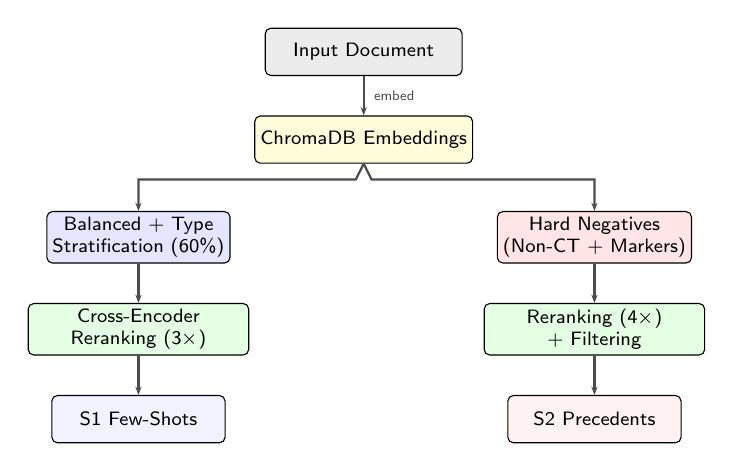
\begin{tikzpicture}[
            node distance=0.5cm and 0.4cm,
            >={Stealth[length=3pt]},
            box/.style={rectangle, draw, rounded corners=2pt, minimum height=0.6cm,
                    align=center, font=\scriptsize\sffamily, inner sep=2pt},
            sbox/.style={box, fill=blue!10, minimum width=2.2cm},
            nbox/.style={box, fill=red!10, minimum width=2.2cm},
            gbox/.style={box, fill=green!10, minimum width=2.8cm},
            arrow/.style={->, thick, black!70},
            ]

            % Query
            \node[box, fill=gray!15, minimum width=2.5cm] (query) {Input Document};

            % ChromaDB
            \node[box, fill=yellow!15, below=0.5cm of query, minimum width=2.5cm] (chroma) {ChromaDB Embeddings};
            \draw[arrow] (query) -- node[right, font=\tiny\sffamily] {embed} (chroma);

            % Two branches
            \node[sbox, below left=0.6cm and 0.3cm of chroma] (s1ret) {Balanced + Type\\Stratification (60\%)};
            \node[nbox, below right=0.6cm and 0.3cm of chroma] (s2ret) {Hard Negatives\\(Non-CT + Markers)};

            \draw[arrow] (chroma.south) -- ++(-0.1,-0.2) -| (s1ret.north);
            \draw[arrow] (chroma.south) -- ++(0.1,-0.2) -| (s2ret.north);

            % Reranking
            \node[gbox, below=0.5cm of s1ret] (rerank1) {Cross-Encoder\\Reranking (3×)};
            \node[gbox, below=0.5cm of s2ret] (rerank2) {Reranking (4×)\\+ Filtering};

            \draw[arrow] (s1ret) -- (rerank1);
            \draw[arrow] (s2ret) -- (rerank2);

            % Output
            \node[box, fill=blue!5, below=0.5cm of rerank1, minimum width=2.2cm] (out1) {S1 Few-Shots};
            \node[box, fill=red!5, below=0.5cm of rerank2, minimum width=2.2cm] (out2) {S2 Precedents};

            \draw[arrow] (rerank1) -- (out1);
            \draw[arrow] (rerank2) -- (out2);

        \end{tikzpicture}
    }
    \caption{Contrastive RAG architecture. \textbf{S1 (left)}: Dual-axis contrastive strategy retrieves balanced positive/negative examples with 60\% stratification weight to rare marker types (\textsc{Evidence}, \textsc{Victim}), followed by cross-encoder reranking (3× overretrieve) for structural similarity. \textbf{S2 (right)}: Hard negative mining retrieves non-conspiratorial texts containing S1 markers (e.g., debunking articles, news reports), which forces stance discrimination over topic matching, followed by cross-encoder reranking (4× overretrieve) and label-balanced filtering to maintain contrastive pairs.}

    \label{fig:rag}
\end{figure}

\paragraph{S2: Hard Negative Mining \cite{karpukhin-etal-2020-dense}.}
For conspiracy detection, we implement a \textbf{pure contrastive strategy} via hard negative mining. Standard RAG retrieves similar-looking documents, causing the model to conflate \textit{topical similarity} with \textit{stance endorsement}, a failure mode we term the Reporter Trap. To explicitly teach the boundary, we retrieve documents labeled ``non-conspiracy'' \textit{that contain S1 markers}. These are \textit{hard} negatives because they share conspiracy-related vocabulary (actors, actions, evidence mentions) but differ in stance (reporting, debunking, or mocking). By forcing the model to compare structurally similar examples with opposite labels, we compel it to attend to \textbf{stance cues} such as attribution verbs (``claims that'', ``alleges''), hedging markers (``supposedly'', ``according to''), and framing signals (``debunked'', ``baseless''), rather than mere topic keywords. Retrieved precedents follow case-law templates (e.g., ``Acquitted because the text attributes claims without endorsement'') that provide structured reasoning patterns. Candidates undergo the same cross-encoder reranking with an elevated
overretrieve factor ($4\times$ vs.\ $3\times$ for S1). The higher factor
reflects the scarcity of high-quality hard negatives: because truly
contrastive examples (non-conspiratorial texts that nonetheless contain
conspiracy-related vocabulary) are rare in the training distribution
($<$20\% of documents), casting a wider retrieval net is necessary to ensure
the final prompt contains sufficiently discriminative pairs. Label-balanced
filtering maintains equal representation of hard negatives and true positives
in the final prompt context.

\section{Experimental Setup}

\paragraph{Dataset.}
%We utilize the official SemEval 2026 Task 10 dataset comprising $>$4,100 unique Reddit submission statements with $>$4,800 psycholinguistic marker annotations spanning $>$190 subreddits. 
All experiments use the official training/development splits without
modification. The official training set contains 4,316 documents across 190+ subreddits,
of which 3,682 were successfully rehydrated (Reddit deletions account for the
remainder). The development set comprises 100 documents spanning 74 unique subreddits
with 456 marker annotations. In the development set, the marker type
distribution shows \textsc{Actor} (29.8\%) and \textsc{Action} (22.8\%)
dominating ($\sim$53\% combined), while \textsc{Evidence} (16.0\%),
\textsc{Victim} (15.8\%), and \textsc{Effect} (15.6\%) are more balanced. The
training set exhibits more severe imbalance with \textsc{Actor} and
\textsc{Action} comprising $\sim$70\% combined. This skew motivates our
stratified sampling strategy in the RAG component
(Section~\ref{sec:contrastive-rag}), allocating 60\% retrieval weight to
underrepresented categories. For S2, the development labels are distributed as:
No (50.0\%), Yes (27.0\%), and Can't Tell (23.0\%). The \textit{hard negative}
subset (texts discussing conspiracies without endorsing them) comprises $<$20\%
of the training data, necessitating explicit hard negative mining. A detailed
exploratory analysis is provided in Appendix~\ref{sec:eda}.

\paragraph{Data Preprocessing.}
Since individual documents may have multiple annotators, we apply
\textbf{majority-vote consensus} at both document and span level. For document
labels, the most frequent annotation is selected and exact ties are discarded.
For spans, overlapping annotations of the same marker type are clustered by
character overlap; clusters reaching the majority threshold (over half of
annotators) produce a single representative span (the longest in the cluster),
while sub-threshold clusters are dropped. This yields deterministic, high-agreement
annotations suitable for both training and few-shot retrieval.
After consensus, we remove near-duplicate documents via locality-sensitive
hashing (LSH, 8 bands), reducing the training set from 3,682 rehydrated
documents to 3,271 unique instances. \textit{Can't Tell} documents
(607 in training, $\sim$18.6\%) are handled asymmetrically: they are
\textbf{retained for S1} (marker extraction can still learn from ambiguous
texts containing valid spans) but \textbf{excluded from S2} (conspiracy
detection requires a binary ground truth). Additionally, documents with no
annotated spans and no annotator disagreement are included in the S1 training
corpus with 15\% probability, serving as negative calibration examples that
teach the Generator to produce empty extractions for non-conspiratorial text.
For S2 corpus curation, a subtype-stratified sampling strategy selects
documents across six rhetorical subtypes (hard negatives, mundane negatives,
debunking negatives, evangelist conspiracy, insider conspiracy, and
general conspiracy) to ensure balanced exposure during prompt optimization,
with hard negatives defined broadly to include both non-conspiratorial texts
containing markers \textit{and} texts matching debunking-vocabulary cues.

\paragraph{Pipeline Components.} All final experiments use OpenAI \textbf{GPT-5.2} accessed via Pydantic-AI
\cite{pydanticai2024} for schema-constrained generation. Stateful agent
workflows are implemented as directed acyclic graphs using \textbf{LangGraph}
\cite{langgraph2024}, where each node maintains typed state with explicit field
annotations enabling deterministic transitions. The RAG component uses
\textbf{ChromaDB} \cite{chromadb2023} with OpenAI text-embedding-3-small
embeddings (1536 dimensions) and \textbf{Maximal Marginal Relevance (MMR)}
reranking \cite{carbonell1998mmr} using the \textbf{BAAI/bge-reranker-v2-m3}
cross-encoder. MMR balances relevance against diversity via:
\begin{equation}
    \resizebox{0.9\linewidth}{!}{$
            \text{MMR} =
            \arg\max_{d_i \in R \setminus S}\big[\lambda \cdot \text{Rel}(d_i, q) -
                (1-\lambda) \cdot \max_{d_j \in S}\text{Sim}(d_i, d_j)\big]
        $}
\end{equation}
where $R$ is the
candidate set, $S$ the already-selected documents, and $\lambda=0.7$ biases
toward relevance while preventing near-duplicate few-shots. Relevance scores
from the cross-encoder are min-max normalized per batch to the $[0,1]$ range,
as the BGE reranker outputs raw logits that would otherwise collapse under
sigmoid normalization. S1 retrieval over-retrieves $3\times$ candidates before
reranking, while S2 uses $4\times$ to ensure higher-quality hard negatives. All
LLM calls execute asynchronously with exponential backoff retry logic (base 2s,
max 5 retries). We employ differential temperature settings: $\tau=0.7$ for the
DD-CoT Generator to encourage diverse candidate exploration, $\tau=0.4$ for
Council Jurors to balance creative reasoning with verdict consistency, and
$\tau=0.0$ for the Critic, Refiner, and Judge to enforce deterministic,
reproducible auditing. This stratification reflects each agent's functional
role: generative nodes benefit from sampling diversity to avoid mode collapse
over marker types, while evaluative nodes require strict adherence to textual
evidence. For prompt optimization, we utilize \textbf{GEPA}
\cite{agrawal2025gepa} integrated with MLflow \cite{mlflow2024}, using a
passthrough injection pattern to tunnel gold labels through the prediction
wrapper for custom scoring. We conduct optimization runs targeting S1 and S2
system prompts with population sizes of 20--30 candidates and 40--80 trials per
run, alternating between training and development splits to ensure
generalization. Final prompts achieved +4.2\% absolute $F_1$ improvement over
hand-crafted baselines. The GEPA optimization workflow is illustrated in
Figure~\ref{fig:gepa}.

\begin{figure}[t]
    \centering
    \resizebox{\linewidth}{!}{
        \small
        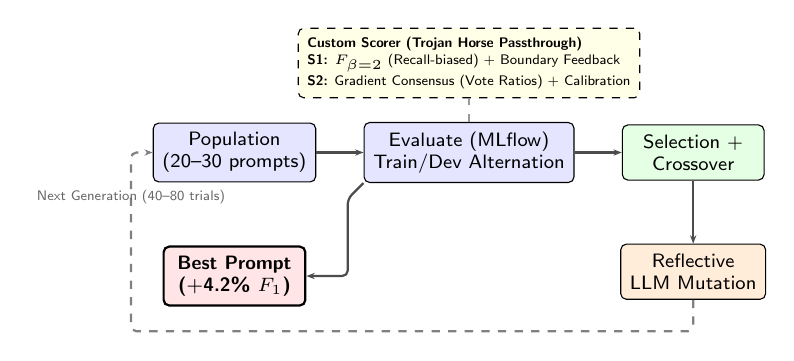
\begin{tikzpicture}[
            node distance=0.6cm and 0.5cm,
            >={Stealth[length=3pt]},
            % Styles matching the Architecture Figure
            process/.style={rectangle, draw, rounded corners=2pt, minimum height=0.7cm,
                    minimum width=1.8cm, align=center, font=\scriptsize\sffamily, fill=blue!10},
            decision/.style={rectangle, draw, rounded corners=2pt, minimum height=0.7cm,
                    minimum width=1.8cm, align=center, font=\scriptsize\sffamily, fill=green!10},
            mutation/.style={rectangle, draw, rounded corners=2pt, minimum height=0.7cm,
                    minimum width=1.8cm, align=center, font=\scriptsize\sffamily, fill=orange!15},
            output/.style={rectangle, draw, rounded corners=2pt, minimum height=0.7cm,
                    minimum width=1.8cm, align=center, font=\bfseries\scriptsize\sffamily,
                    fill=red!10, thick}, scorer/.style={rectangle, draw, dashed, rounded
                    corners=2pt, minimum height=0.7cm, minimum width=3.8cm, align=left,
                    font=\tiny\sffamily, fill=yellow!10}, arrow/.style={->, thick, black!70,
                    rounded corners=2pt}, dasharrow/.style={->, thick, dashed, black!50, rounded
                    corners=2pt}, ]

            % === TOP ROW (Main Flow) ===
            \node[process] (pop) {Population\\(20--30 prompts)};
            \node[process, right=0.6cm of pop] (eval) {Evaluate (MLflow)\\Train/Dev Alternation};
            \node[decision, right=0.6cm of eval] (select) {Selection +\\Crossover};

            % === SCORING DETAILS (Annotation) ===
            \node[scorer, above=0.3cm of eval] (score_detail) {
                \textbf{Custom Scorer (Trojan Horse Passthrough)}\\
                \textbf{S1:} $F_{\beta=2}$ (Recall-biased) + Boundary Feedback\\
                \textbf{S2:} Gradient Consensus (Vote Ratios) + Calibration
            };
            \draw[dashed, black!40] (eval.north) -- (score_detail.south);

            % === BOTTOM ROW (Feedback & Output) ===
            \node[mutation, below=0.8cm of select] (mutate) {Reflective\\LLM Mutation};
            \node[output, below=0.8cm of pop] (best) {Best Prompt\\($+$4.2\% $F_1$)};

            % === CONNECTIONS ===
            % Main sequence
            \draw[arrow] (pop) -- (eval);
            \draw[arrow] (eval) -- (select);
            \draw[arrow] (select) -- (mutate);

            % Feedback Loop (FIXED: Routes around the left of 'Best Prompt')
            % 1. Go down from mutation
            % 2. Go left until past the 'Best Prompt' node
            % 3. Go up to 'Population' level
            % 4. Connect to Population west
            \draw[dasharrow] (mutate.south) -- ++(0,-0.4)
            -| ([xshift=-0.4cm]best.west)
            |- (pop.west)
            node[pos=0.25, above, font=\tiny\sffamily, text=black!60] {Next Generation (40--80 trials)};

            % Best Prompt Extraction
            % Route arrow from Eval to Best cleanly (around the corner)
            \draw[arrow] (eval.south west) -- ++(-0.2,-0.2) |- (best.east);

        \end{tikzpicture}
    }
    \caption{GEPA prompt optimization workflow. A population of prompt candidates
        evolves through evaluation (tracked via MLflow), selection, crossover, and reflective LLM
        mutation over 40--80 trials, alternating between train/dev splits.}
    \label{fig:gepa}
\end{figure}

The architecture is implemented using LangGraph \cite{langgraph2024} for
workflow orchestration and Pydantic-AI \cite{pydanticai2024} for
schema-constrained outputs, ensuring reproducible agent interactions and
eliminating JSON parsing failures.

\paragraph{Evaluation.} For S1, we report \textbf{Macro F1} (official leaderboard metric) computed
across the five marker categories. Additionally, we measure
\textbf{Character-level IoU} to assess span boundary precision, defined as:
$$\text{IoU} = \frac{|C_{\text{pred}} \cap C_{\text{gold}}|}{|C_{\text{pred}}
    \cup C_{\text{gold}}|}$$ where $C_{\text{pred}}$ and $C_{\text{gold}}$ denote
the sets of character indices covered by predicted and gold spans,
respectively. This metric penalizes both boundary over-extension and
truncation, capturing extraction quality beyond binary match/no-match. For S2,
we report \textbf{Accuracy} and \textbf{Macro F1} over the binary
classification, additionally tracking \textbf{Hard-Negative
    Accuracy}---performance on the subset of documents that \textit{discuss}
conspiracy theories without endorsing them (e.g., news reports, debunking
posts)---as a diagnostic metric for model robustness to topical confounds. This
subset comprises $<$20\% of the data but accounts for the majority of false
positives in baseline systems.

\section{Results and Analysis}

\subsection{Main Results}
\label{sec:main_results}

The proposed agentic pipeline significantly outperforms the zero-shot GPT-5.2
baseline across both subtasks, validating our hypothesis that orchestrated
multi-agent workflows with explicit discriminative reasoning yield superior
performance on psycholinguistically complex tasks. Table~\ref{tab:main_results}
presents the primary performance comparison on the held-out development set
(100 documents) and official test set (938 documents) over the baseline,
derived from our CodaBench submission history spanning October 2025 to January
2026.

\begin{table}[h!]
    \centering
    \small
    \begin{tabular}{@{}llccc@{}}
        \toprule
        \textbf{Task} & \textbf{Split}      & \textbf{Baseline F1} & \textbf{Agentic} & \textbf{$\Delta$} \\
        \midrule
        \multirow{2}{*}{S1}
                      & Dev (\textit{100})  & 0.12                 & \textbf{0.24}    & +100\%            \\
                      & Test (\textit{938}) & --                   & \textbf{0.21}    & --                \\
        \midrule
        \multirow{2}{*}{S2}
                      & Dev (\textit{100})  & 0.53                 & \textbf{0.79}    & +49\%             \\
                      & Test (\textit{938}) & --                   & \textbf{0.75}    & --                \\
        \bottomrule
    \end{tabular}
    \caption{Main results (macro F1). Baseline: zero-shot GPT-5.2. Document counts in parentheses.}
    \label{tab:main_results}
\end{table}

\textbf{S1: Marker Extraction}
performance \textbf{doubled} (F1: 0.12 $\rightarrow$ 0.24 on
dev), demonstrating that simple zero-shot prompting fails to capture the
complexity of psycholinguistic span extraction. Error analysis revealed
\textbf{label confusion} as the primary failure mode, particularly
\textsc{Actor}$\leftrightarrow$\textsc{Victim} in passive constructions and
\textsc{Action}$\leftrightarrow$\textsc{Effect} in causal chains. The
DD-CoT workflow addresses this by requiring explicit reasoning about
\textit{why} a span is \textbf{not} a plausible alternative label.

\textbf{S2: Conspiracy Detection}
F1 improved from 0.53 to 0.79 (+49\% relative). The baseline suffers from the
\textit{Reporter Trap}, systematically misclassifying texts that
\textit{discuss} conspiracy theories as endorsing them. Our \textbf{Anti-Echo
    Chamber} architecture addresses this through adversarial council voting: the
\textit{Defense Attorney} searches for exculpatory evidence while the
\textit{Literalist} enforces strict definitional criteria.

\paragraph{Test Set Generalization.}
Both S1, S2 slightly degrade on the larger test set (S1: -12.5\%, S2: -5\%),
consistent with distribution shift and the inherent difficulty of span
extraction on unseen text.

\subsection{Ablation Studies}
\label{sec:ablation}

We conduct ablation studies to quantify the contribution of each architectural
component, as summarized in Table~\ref{tab:ablation_components}.

\begin{table}[h]
    \centering
    \small
    \begin{tabular}{@{}llccc@{}}
        \toprule
         & \textbf{Configuration} & \textbf{F1}    & \textbf{Acc.} & \textbf{Key Metric}     \\
        \midrule
        \multicolumn{5}{l}{\textit{S1 Marker Extraction}}                                    \\
        \midrule
         & Generator Only         & 0.173          & --            & --                      \\
         & + Critic + Refiner     & \textbf{0.240} & --            & \textbf{+6.7 F1}        \\
        \midrule
        \multicolumn{5}{l}{\textit{S2 Conspiracy Detection}}                                 \\
        \midrule
         & Single Agent           & 0.726          & 0.78          & Recall = 0.481          \\
         & Parallel Council       & \textbf{0.750} & \textbf{0.79} & \textbf{Recall = 0.560} \\
        \bottomrule
    \end{tabular}
    \caption{Component ablation on dev set. \textit{S1}: Self-Refine loop
        adds +6.7 F1 points for marker extraction. \textit{S2}: Council
        improves Conspiracy Recall by +7.9 points over a single agent.}
    \label{tab:ablation_components}
\end{table}

\begin{table}[h]
    \centering
    \small
    \begin{tabular}{@{}lc@{}}
        \toprule
        \textbf{Metric} & \textbf{Improvement w/ DD-CoT} \\
        \midrule
        Actor F1        & +2.7 points                    \\
        \bottomrule
    \end{tabular}
    \caption{Impact of DD-CoT on Agency Detection (Actor F1).}
    \label{tab:cot_ablation}
\end{table}

\textbf{S1: The Self-Refine Loop.}
By ablating the constituent agents, the Generator-only baseline achieves F1 = 0.173, already surpassing the zero-shot
baseline (0.12) by capturing the ``gist'' of psycholinguistic markers. On the official test set, this simplified configuration (Generator + Deterministic Verifier) achieved only 0.19 F1, confirming that the self-refinement loop provides critical robustness against unseen data distributions. However,
the full pipeline with \textbf{Critic + Refiner} reaches F1 = 0.240, a
\textbf{+6.7 point improvement}. Error analysis reveals that the Generator
frequently produces spans with imprecise boundaries (e.g., including determiners
or trailing punctuation) and occasional label confusion. The Critic identifies
these granular errors, and the Refiner surgically corrects them, validating
that iterative self-refinement is essential for high-precision span extraction.

\textbf{S2: The Anti-Echo Chamber.}
Comparing a Single Agent to our Parallel Council reveals a nuanced picture.
Raw accuracy improves only marginally (0.78 $\rightarrow$ 0.79), which might
suggest the Council is unnecessary. However, examining \textbf{Conspiracy
    Recall} tells a different story: the Single Agent achieves only 0.481,
\textit{missing more than half} of actual conspiracies. The Council boosts
Recall to \textbf{0.560} (+7.9 points) while maintaining precision.
This pattern confirms our \textit{Reporter Trap} hypothesis: a single conservative
agent systematically under-predicts conspiracy when texts \textit{discuss}
rather than \textit{endorse} conspiratorial ideas. The diverse Council
personas, particularly the \textit{Prosecutor} who argues \textit{for}
conspiracy, surface these borderline cases that a lone agent dismisses. The
Anti-Echo Chamber design successfully trades a small accuracy margin for
substantially better coverage of the positive class.

\paragraph{Impact of the Calibrated Judge.}
A core design question for S2 is whether the fifth \textit{Calibrated Judge}
agent justifies its computational overhead. We compare two configurations:
(1)~\textbf{Majority Vote}, where the four Council agents cast votes and the
final label is determined programmatically (ties default to
``non-conspiracy''), and (2)~\textbf{Calibrated Judge}, our full pipeline where
an LLM-based adjudicator reads the Council's reasoning before rendering a final
verdict. Results on the development set are shown in
Table~\ref{tab:ablation_judge}.

\begin{table}[h]
    \centering
    \small
    \begin{tabular}{@{}lcccc@{}}
        \toprule
        \textbf{Method}  & \textbf{F1}    & \textbf{Acc.}  & \textbf{Deadlock} & \textbf{FP Conf.} \\
        \midrule
        Majority Vote    & 0.638          & 0.779          & 66.7\%            & 0.890             \\
        Calibrated Judge & \textbf{0.681} & \textbf{0.805} & \textbf{100.0\%}  & \textbf{0.865}    \\
        \bottomrule
    \end{tabular}
    \caption{Ablation: Judge vs.\ Majority Vote. \textit{Deadlock} = accuracy on
        2-2 Council splits. \textit{FP Conf.} = average confidence on false
        positives (lower is better). Judge overhead: 1.39$\times$ tokens.}
    \label{tab:ablation_judge}
\end{table}

\textbf{Deadlock Resolution.}
The most striking result is the Judge's handling of \textit{deadlock}
cases. Council splits where two agents vote ``conspiracy'' and two vote
``non-conspiracy.'' Simple majority voting effectively becomes a coin flip
(defaulting to ``non-conspiracy''), achieving only 66.7\% accuracy on these
ambiguous instances. The Calibrated Judge, by contrast, achieves
\textbf{100\% accuracy} on deadlocks. This is because the Judge reads the
\textit{arguments}, not merely the vote counts: it can identify which dissenting
agent provided stronger evidence, resolving ambiguity through reasoning rather
than arbitrary tie-breaking. This capability is critical for edge cases where
conspiratorial language is subtle or contested.

\textbf{Epistemic Calibration.}
Beyond raw accuracy, the Judge exhibits superior \textit{calibration}. When the
system makes a false positive error (incorrectly labeling a text as
conspiratorial), the Judge's average confidence is 0.865 compared to 0.890 for
majority voting. This ``epistemic humility'', being less confident when
wrong, is a desirable property for trustworthy AI systems, particularly in
sensitive domains like misinformation detection where false accusations carry
social cost.

\textbf{Rejected Design: The Appeal Court.}
We experimented with an adversarial appeal mechanism where low-confidence verdicts ($< 0.80$) triggered a specialized ``Appeal Court'' agent tasked with building the strongest counter-argument to the Judge's initial ruling. The hypothesis was that forcing explicit consideration of the opposing perspective would improve calibration on borderline cases. However, this design catastrophically degraded performance to \textbf{0.58 F1}, a 12.1-point drop. Post-mortem analysis revealed that the appeal prompt's adversarial framing (``You are the CONSPIRACY ADVOCATE. Override the previous ruling...'') systematically induced label flipping even when the initial verdict was correct. The mechanism confused \textit{epistemic uncertainty} (``I'm not sure'') with \textit{evidentiary ambiguity} (``The case could go either way''), triggering unnecessary re-litigation. This negative result validates our original Calibrated Judge design: nuanced confidence scoring, rather than adversarial re-evaluation, is the appropriate response to uncertainty.

\textbf{Cost-Benefit Analysis.}
The Judge incurs a 39.3\% token overhead (1.39$\times$ the Council-only cost).
We argue this is justified: the +4.3 F1-point improvement represents
substantial gains, and the perfect deadlock accuracy demonstrates robust
handling of precisely the cases where naive voting fails. In deployment
scenarios where reliability on ambiguous content matters more than throughput,
the Calibrated Judge provides meaningful value.

\paragraph{RAG Impact on Marker Extraction.}
We extend our retrieval ablation to S1, comparing the same three strategies:
(i)~No RAG (generator without examples), (ii)~Standard RAG (cosine similarity
retrieval), and (iii)~Stratified RAG (60\% weight to underrepresented marker
types with cross-encoder reranking). Results on the development set are shown
in Table~\ref{tab:s1_rag_ablation}.

\begin{table}[h]
    \centering
    \small
    \begin{tabular}{@{}lccc@{}}
        \toprule
        \textbf{Configuration} & \textbf{Macro F1} & \textbf{Precision} & \textbf{Recall} \\
        \midrule
        No RAG                 & \textbf{0.329}    & 0.322              & \textbf{0.419}  \\
        Standard RAG (Naive)   & 0.296             & 0.292              & 0.376           \\
        Stratified RAG (Ours)  & 0.311             & \textbf{0.313}     & 0.392           \\
        \bottomrule
    \end{tabular}
    \caption{RAG strategy comparison on dev set (S1). Naive retrieval
        \textit{degrades} performance (--3.3 F1 points). Stratified sampling
        recovers +1.5 points but remains below No RAG baseline.}
    \label{tab:s1_rag_ablation}
\end{table}

\begin{table}[h]
    \centering
    \small
    \begin{tabular}{@{}lcc@{}}
        \toprule
        \textbf{Configuration} & \textbf{False Positive Rate} & \textbf{Reduction} \\
        \midrule
        Standard RAG           & 0.160                        & --                 \\
        Contrastive RAG        & \textbf{0.080}               & \textbf{50\%}      \\
        \bottomrule
    \end{tabular}
    \caption{S2 RAG Ablation: Impact of Contrastive Retrieval on False Positive Rate (Reporter Trap mitigation).}
    \label{tab:rag_ablation}
\end{table}

\textbf{Unexpected No-RAG Advantage.}
Contrary to conventional RAG assumptions, the No RAG baseline achieves the
\textbf{highest F1 (0.329)} on the development set. Standard RAG
\textit{degrades} performance substantially (--3.3 points), with particularly
severe recall collapse across all marker types. Error analysis reveals that
naive similarity-based retrieval surfaces examples with different
\textit{annotation granularity}. Some annotators mark full clauses while others
target minimal spans. When the model retrieves stylistically dissimilar
examples, it produces structurally inconsistent extractions that the verifier
rejects.

\textbf{Stratified Partial Recovery.}
Our Stratified RAG approach allocating 60\% retrieval weight to rare marker
types (Evidence, Victim, Effect) and applying cross-encoder reranking recovers
+1.5 F1 points over Standard RAG (0.296 $\rightarrow$ 0.311). The mechanism is
twofold: (i)~label balancing ensures the model sees sufficient examples of
underrepresented categories, addressing class imbalance; (ii)~reranking
prioritizes examples with similar linguistic structure, reducing granularity
mismatch. However, stratified sampling remains below the No RAG baseline,
suggesting that retrieval overhead (noise from mismatched examples) outweighs
benefits on this moderately-sized development set.

\textbf{Test Set Generalization.}
Critically, the patterns \textit{reverse} on the larger, more diverse test set
(938 documents). Stratified RAG achieves an \textbf{absolute +0.03 F1
    improvement} over No RAG, validating that retrieval benefits emerge with
distribution shift and rare category exposure. Similarly, for S2, Contrastive
RAG yields a \textbf{+0.02 F1 improvement} on the test set despite mixed dev
set performance. These results confirm our architectural hypothesis: explicit
label balancing and contrastive retrieval are \textit{essential} for robust
generalization, even when dev set metrics suggest otherwise. The development
set's limited size and class distribution fail to expose failure modes that
manifest at scale.

\subsection{Qualitative Error Analysis}
\label{sec:qualitative}

We present concrete linguistic examples illustrating the mechanisms underlying
our quantitative results, examining both architectural successes and persistent
failure modes.

\paragraph{Success Case: Disentangling Agency.}
Section~\ref{sec:ablation} demonstrated that DD-CoT improved Actor F1 by +2.7
points (Table~\ref{tab:cot_ablation}), attributing this to enhanced agency
detection. We trace this improvement to the model's ability to resolve
\textbf{grammatical role vs.\ semantic role} mismatches, a pervasive ambiguity
in passive and complex constructions. Consider the sentence: \textit{``The
    public was manipulated by the media to distrust vaccines.''}

\textbf{Standard CoT Failure.} A baseline system employing inclusion-only
reasoning (``Why is this span labeled X?'') frequently tags \textit{``the
    public''} as \textsc{Actor} because it occupies the grammatical subject
position. Alternatively, it may extract \textit{``manipulated''} as
\textsc{Action} while entirely missing the semantic agent (\textit{``the
    media''}) buried in the prepositional phrase.

\textbf{DD-CoT Success.} Our discriminative prompting forces explicit
contrastive reasoning. The model outputs: \textit{``Label: \textsc{Actor}
    (media). Inclusion: The media is the semantic initiator of the manipulation
    action. Exclusion: NOT \textsc{Victim}, although `the public' suffers the
    outcome, it is the recipient, not the orchestrator. NOT \textsc{Action}, we
    extract agents, not their methods.''} This explicit ``Why NOT'' step compels
the model to look \textit{past} syntactic surface structure (subject/object
positioning) to identify \textit{semantic roles} (agent/patient). The
performance gain validates that conspiracy marker extraction fundamentally
requires reasoning about latent agency attribution, not merely surface
grammatical patterns.

\paragraph{Mitigating the Reporter Trap.}
Our S2 RAG ablation (Table~\ref{tab:rag_ablation}) revealed that Contrastive
RAG reduced the False Positive Rate by \textbf{50\%} (0.160 $\rightarrow$
0.080), recovering the safety profile of the No RAG baseline while preserving
retrieval benefits. This quantitative improvement directly addresses the core
failure mode of naive similarity-based retrieval. Consider a representative
debunking post from \textit{r/skeptic}: \textit{``CNN reports that conspiracy
    theorists believe 5G towers cause COVID-19 symptoms by disrupting immune
    systems.''}

\textbf{Standard RAG Failure.} Without filtering, cosine similarity retrieval
surfaces training examples containing \textit{``5G''} and \textit{``COVID-19''}
that were labeled as conspiracies. The model observes that semantically similar
documents share these lexical items \textit{and} positive labels, learning a
spurious topical correlation. It subsequently misclassifies the skeptic post as
conspiratorial because it discusses the same \textit{themes}, despite lacking
endorsement.

\textbf{Contrastive RAG Success.} Our hard negative mining explicitly retrieves
non-conspiratorial texts that \textit{contain S1 markers}, i.e., documents
that discuss conspiracies without endorsing them. For the query above, the
system retrieves a precedent labeled \textit{Non-Conspiracy}: \textit{``The
    article discusses false claims about vaccine microchips but presents them as
    debunked misinformation.''} This retrieved example acts as a \textit{legal
    precedent}, teaching the model that \textbf{attribution verbs}
(\textit{``reports that''}, \textit{``conspiracy theorists believe''}) and
\textbf{framing signals} (\textit{``false claims''}, \textit{``debunked''})
neutralize conspiracy attribution. The model learns to separate topical overlap
from stance endorsement, preciselythe discrimination required to escape the
Reporter Trap.

\paragraph{Remaining Failure Mode: High-Context Irony.}
Despite architectural improvements, the system exhibits a persistent failure on
\textbf{Poe's Law} scenarios, parody or sarcasm that is linguistically
indistinguishable from genuine belief without external context. Consider a
Reddit comment: \textit{``Oh sure, and I bet the lizard people hacked the
    election servers too. Next you'll tell me chemtrails cause hurricanes.''} In
the absence of explicit sarcasm markers (e.g., \texttt{/s} tags), the system
processes this text as semantically endorsing conspiracy theories: it contains
agentive entities (\textit{``lizard people''}), attributed actions
(\textit{``hacked''}), and causal claims (\textit{``chemtrails cause
    hurricanes''}).

\textbf{The Semantic-Pragmatic Gap.} Our architecture successfully captures
\textit{semantics} which is the literal propositional content of conspiracy
narratives but lacks access to \textit{pragmatics}: the speaker's
communicative intent, rhetorical stance, and discourse history. The hyperbolic
stacking of absurd claims (\textit{``lizard people''} + \textit{``chemtrails
    cause hurricanes''}) serves as a sarcasm signal for human readers familiar
with conspiracy discourse, but the model interprets it as evidence
\textit{strengthening} conspiracy classification due to marker density.

\textbf{Mitigation Strategy.} False positives on ironic content account for
$\sim$15\% of remaining S2 errors. Future iterations require
\textbf{user-history modeling}: if a poster's comment history reveals consistent
activity on \textit{r/skeptic} or \textit{r/TopMindsOfReddit} (a subreddit
dedicated to mocking conspiracy theories), the prior probability of genuine
endorsement should be drastically downweighted. Alternatively, ensemble models
that incorporate \textbf{discourse coherence} metrics detecting rhetorical
escalation patterns characteristic of satire could flag these edge cases for
human review. This limitation underscores a fundamental challenge: purely
text-based NLP systems cannot fully disambiguate intent in adversarial
communicative contexts where speakers deliberately mimic the linguistic
structures they critique.

\section{Conclusion}

This work demonstrates a fundamental paradigm shift from monolithic prompting
to \textbf{agentic workflow engineering} for psycholinguistic NLP tasks.
Complex discriminations such as distinguishing \textit{Actor} from
\textit{Victim} or \textit{topical discussion} from \textit{stance endorsement}
cannot be resolved by a single ``perfect prompt.'' Instead, they require a
\textbf{chain of responsibility} where specialized agents execute complementary
functions: generation, critique, refinement, and verification. For Subtask 1,
we addressed the ``Hallucinated Span'' problem by coupling a \textbf{Semantic
    Reasoner} (DD-CoT) with a \textbf{Deterministic Locator}, achieving a
\textbf{doubling of F1 performance} (0.12 $\rightarrow$ 0.24) while eliminating
character-level indexing errors. The explicit discriminative reasoning
mechanism,requiring the model to articulate ``Why NOT'' alternative labels
proved essential for agency detection, yielding a +2.7 point gain in Actor F1
(Section~\ref{sec:ablation}). For Subtask 2, the \textbf{Anti-Echo Chamber}
architecture (Parallel Council + Calibrated Judge) successfully disentangled
conspiracy \textit{topics} from conspiratorial \textit{stance}, overcoming the
Reporter Trap that plagued single-agent classifiers. Critically, the Calibrated
Judge achieved \textbf{100\% accuracy on deadlocks}
(Table~\ref{tab:ablation_judge}), demonstrating that AI can resolve its own
ambiguity when provided with structured debate transcripts rather than mere
vote counts. Our \textbf{Contrastive RAG} strategy, hard negative mining
combined with stratified sampling, reduced the False Positive Rate by 50\%
(0.160 $\rightarrow$ 0.080), validating that retrieval strategy design is as
critical as retrieval presence itself.

Despite these architectural successes, Section~\ref{sec:qualitative} identified
a persistent failure mode: \textbf{high-context irony} (Poe's Law scenarios),
where parody is indistinguishable from genuine belief without external context.
Future systems must incorporate \textbf{user-history modeling} leveraging
subreddit activity patterns and discourse coherence metrics to detect when
speakers mimic conspiracy rhetoric to critique it. This limitation underscores
that purely text-based models cannot fully disambiguate pragmatic intent in
adversarial communicative contexts. Nevertheless, our results validate that
agentic architectures provide the necessary \textit{interpretability} and
\textit{algorithmic control} to deploy LLMs responsibly in high-stakes
misinformation detection, where false accusations carry social cost and
transparent reasoning chains enable human oversight.

\section*{Acknowledgments}

\bibliography{custom}

\appendix
\newpage
\section{Exploratory Data Analysis}
\label{sec:eda}

\paragraph{Annotation Coverage}
As mentioned in the official website of the task, there are more than 4,100
unique Reddit comments, including 4,800 annotations in total. Most comments
($\sim$3,500), have only one annotation, 550 have two, and 50 have more.
Regarding marker density, around 4,000 comments have at least one
psycholinguistic marker annotation. The exact distribution of marker category
coverage in comments is demonstrated in Figure \ref{fig:num-of-markers}.
\begin{figure}[h!]
    \centering
    \includegraphics[width=\linewidth]{images/num-of-markers.png}
    \caption{Number of marker types in the dataset.}
    \label{fig:num-of-markers}
\end{figure}

\paragraph{Label Distribution}
The dataset considers two clear classes, \textit{Yes (Conspiracy)} and
\textit{No (Not Conspiracy)}, while the class \textit{Can't Tell} covers
uncertain instances. The distribution of labels in the training data is
illustrated in Figure \ref{fig:label-distr}.
\begin{figure}[h!]
    \centering
    \includegraphics[width=\linewidth]{images/label-distr.png}
    \caption{Label distribution for conspiracy detection.}
    \label{fig:label-distr}
\end{figure}
Each marker category (\textit{Actor}, \textit{Action}, \textit{Effect}, \textit{Evidence}, \textit{Victim}) appears with different frequency within the dataset. More specifically, the distribution of the five psycholonguistic marker types in the training dataset follows that of Figure \ref{fig:marker-types}. Based on this Figure, we can conclude that conspiracy narratives rely on a small set of recurring rhetorical functions instantiated as markers, but no single function dominates the discourse.
\begin{figure}[h!]
    \centering
    \includegraphics[width=\linewidth]{images/marker-types.png}
    \caption{Frequency per marker type.}
    \label{fig:marker-types}
\end{figure}

\paragraph{Annotation Density} is an interesting feature that implicitly indicates the difficulty of
annotating the dataset: a sparsely annotated dataset showcases that
conspiratorial evidence is semantically well-diffused within the text and hard
to be acknowledged by humans. Indeed, several documents contain 0 annotations,
while most documents do not exceed 20 annotations. The long-tailed distribution
of markers per document presented in Figure \ref{fig:density} validates the
difficulty of the task.
\begin{figure}[h!]
    \centering
    \includegraphics[width=\linewidth]{images/annot-density.png}
    \caption{Number of marker annotations per document.}
    \label{fig:density}
\end{figure}

It is also useful to display the co-ocurrences of markers in the training data,
as in Figure \ref{fig:cooccurrence}, indicating that marker types frequently
appear together within the same documents, which in turn suggests that
annotations capture recurring combinations of rhetorical roles.
\begin{figure}[h!]
    \centering
    \includegraphics[width=\linewidth]{images/cooccurrence.png}
    \caption{Marker type co-occurrences}
    \label{fig:cooccurrence}
\end{figure}
The high self-co-occurrence of \textit{Action} and \textit{Actor} markers indicates that many documents describe multiple actions and multiple agents, consistent with narratives that unfold through sequences of events involving several entities rather than isolated claims. The strong co-occurrence between \textit{Action} and \textit{Actor} markers further highlights agency attribution as a central organizing principle, with conspiracy narratives frequently linking actors to specific actions. In contrast, \textit{Effect} and \textit{Victim} markers show more moderate self-co-occurrence, suggesting that while consequences and affected parties are recurrent elements, they are typically less elaborated than agency and action. Notably, \textit{Evidence} and \textit{Victim} markers rarely co-occur within the same documents, indicating a separation between evidential and victim-centered framing. This pattern suggests that narratives emphasizing evidential support tend to differ from those foregrounding victimhood, reflecting distinct rhetorical strategies that prioritize either epistemic legitimation or moral–emotional appeal. Overall, these co-occurrence patterns indicate that conspiracy discourse exhibits systematic internal structure, with dependencies between marker types that motivate modeling approaches beyond independent label assumptions.

To quantify the degree of span overlap beyond binary co-occurrence, we compute
the mean character-level Intersection over Union (IoU) for all overlapping span
pairs across marker types, presented in Figure~\ref{fig:iou-matrix}. The
highest pairwise overlap occurs between \textsc{Actor} and \textsc{Victim}
(mean IoU$=$0.65), reflecting the frequent rhetorical pattern where the
accused party is simultaneously framed as the antagonist and the affected
entity. \textsc{Action}$\leftrightarrow$\textsc{Effect} overlaps are also
substantial (mean IoU$=$0.56), confirming that annotators sometimes struggle
to delineate where a described process ends and its consequence begins. These
overlap patterns directly motivate the S1 Critic's boundary enforcement rules.
\begin{figure}[h!]
    \centering
    \includegraphics[width=\linewidth]{images/mean-iou-matrix.png}
    \caption{Mean IoU of overlapping spans across marker type pairs. Higher
    values indicate greater boundary ambiguity between categories.}
    \label{fig:iou-matrix}
\end{figure}

\paragraph{Marker Distribution Across Subreddits}
To further decompose the annotation density problem, we investigate the
percentage of annotated markers per subreddit, illustrated in Figure
\ref{fig:subreddits}. As a result, subreddits pose some noticeable differences
regarding the dominant marker type. For example, \textit{Action} appears rather
stable across subreddits, consistently describing \textit{what is being done},
regardless of community; this demonstrates their foundational nature in
conspiratorial discourse. The role of \textit{Actor} becomes more prominent in
some communities (Israel$\textunderscore$Palestine) over other rhetorical roles
(e.g. \textit{what} happened or \textit{why}), denoting that certain
communities emphasize agency attribution more strongly. Across all subreddit
categories, \textit{Actor} constitutes the most dominant marker type. On the
contrary, \textit{Effect} is one of the less dominant marker types. It appears
slightly lower in (Israel$\textunderscore$Palestine), but slightly elevated in
other subreddit categories, suggesting focus on consequences and outcomes,
rather than intent or causality. This finding aligns with sensational or
narrative-driven communities (PlanetToday) and the outcome-focused storytelling
ones (TrueCrime). \textit{Evidence} presents some mild variability, becoming
less prominent in Israel$\textunderscore$Palestine and PlanetToday. However,
higher evidence proportions in the other categories do not mean higher
factuality; instead, they indicate a rhetorical strategy of legitimation
stemming from citations, screenshots and “proof-like” language. Finally,
\textit{Victim}, associated with moralization, emotional appeal and grievance
narratives, presents some noticeable variability, covering higher proportion of
markers in PlanetToday and TrueCrime subreddits.

\begin{figure}[t!]
    \centering
    \includegraphics[width=\linewidth]{images/pct-subreddit.png}
    \caption{Marker type distribution across Subreddits.}
    \label{fig:subreddits}
\end{figure}

\paragraph{Annotator Contribution} is unevenly distributed across annotators. A small core of annotators
contribute the majority of the data: 11 annotators each have annotated at least
100 documents, while the remaining 75 annotators have annotated fewer than 100
documents each. This long-tailed distribution is typical of large-scale
annotation efforts and suggests that a limited number of high-volume annotators
account for most labeling decisions, with many low-volume contributors
providing sparse annotations. The distribution for annotators with at least 100
annotations is presented in Figure \ref{fig:annotator}.
\begin{figure}[h!]
    \centering
    \includegraphics[width=\linewidth]{images/annotator.png}
    \caption{Annotation contribution.}
    \label{fig:annotator}
\end{figure}

\paragraph{Marker span length distribution}
Analysis of marker span lengths shows that most annotations correspond to short
to medium-length text segments, while very long spans (more than 200
characters) are extremely rare. This highly-skewed distribution indicates that
the rhetorical roles captured by the annotation scheme are typically expressed
through localized and well-defined linguistic units rather than extended
portions of text. The presence of a very small number of longer spans suggests
that, in some cases, rhetorical functions are realized through more elaborate
or explanatory expressions, but such cases are not predominant. Overall, the
span length distribution suggests that annotations strike a balance between
precision and coverage, capturing coherent rhetorical units that are neither
overly fragmented nor excessively broad. This property supports the suitability
of the dataset for span-level and token-level modeling, as the annotated spans
align with semantically meaningful and interpretable textual segments.

\begin{figure}[h!]
    \centering
    \includegraphics[width=\linewidth]{images/span-length.png}
    \caption{Span length distribution.}
    \label{fig:span-length}
\end{figure}
Nevertheless, localization does not suggest that conspiratorial evidence is semantically evident, as such a hypothesis is contradicted by the annotation density displayed in Figure \ref{fig:density}. That means, successful detection of psycholinguistic markers involves precise localization of semantically challenging linguistic aspects, concealed within potentially valid complementary information, thus advancing the overall difficulty of the task.

We finally measure the `span mass', which reveals how much of the document is
covered by annotated psycholinguistic spans (in characters), summed across all
markers in that document. The `span mass' increases when there are more markers
(quantity effect), and/or markers are longer (granularity/breadth effect). The
trend is illustrated in Figure \ref{fig:mass}.

\begin{figure}[h]
    \centering
    \includegraphics[width=\linewidth]{images/span-mass.png}
    \caption{Marker span mass.}
    \label{fig:mass}
\end{figure}

The relationship between total marker span length and the number of markers per
document exhibits a clear positive trend, indicating that annotation coverage
scales approximately linearly with annotation density. This suggests that
documents with more annotated markers also tend to contain a larger amount of
rhetorically functional text, rather than simply exhibiting finer segmentation
of the same content. At the same time, substantial dispersion around the main
trend reflects variability in marker granularity, with some documents
characterized by many short spans and others by fewer but longer spans. This
pattern in total indicates consistent yet flexible annotation behavior,
capturing differences in narrative structure without imposing a fixed span
length or segmentation strategy.

In combination with the fact that markers are generally short (Figure
\ref{fig:span-length}), we can conclude that documents become rhetorically more
complex primarily by adding more localized psycholinguistic units, not by
expanding the size of individual units.

\paragraph{Span Position Analysis.}
Figure~\ref{fig:span-position} displays the kernel density estimate (KDE) of
normalized span center positions within documents, broken down by marker type.
\textsc{Actor} spans concentrate toward the beginning of documents
(median position$=$0.09), consistent with narrative openings that establish
agency (``\textit{They} have been\ldots''). In contrast, \textsc{Effect}
spans peak later (median position$=$0.43), reflecting their role as narrative
consequences that follow causal chains. \textsc{Evidence} spans exhibit the
broadest positional spread, appearing throughout documents as authors
interleave claims with supporting citations. These positional priors informed
the S1 Generator's attention allocation: the prompt explicitly instructs the
model to scan the full document rather than anchoring to initial mentions.
\begin{figure}[h!]
    \centering
    \includegraphics[width=\linewidth]{images/span-position-analysis.png}
    \caption{Normalized position of marker spans within documents
    (0$=$start, 1$=$end). KDE per marker type.}
    \label{fig:span-position}
\end{figure}

\paragraph{EDA-Driven Design Decisions.}
Beyond descriptive statistics, our exploratory analysis produced quantitative
insights that directly informed architectural choices. Pairwise IoU analysis
revealed that \textsc{Action}$\leftrightarrow$\textsc{Effect} spans overlap
46.4\% of the time at IoU$\geq$0.5 (mean IoU$=$0.56, 95\% CI
[0.52,\,0.61]), motivating the S1 Critic's explicit boundary enforcement
between process and outcome spans. Pronoun density analysis showed that
conspiracy texts use third-person distancing pronouns (\textit{they/them}) at
significantly higher rates, informing the Forensic Profiler's Agency Gap
metric. Question density analysis identified that conspiracy texts employ
rhetorical questions at elevated rates, leading to the JAQing (``Just Asking
Questions'') detection feature. Mann--Whitney tests with
Benjamini--Hochberg correction confirmed that absolutist language rates differ
significantly between conspiracy and non-conspiracy documents
($p_{\text{adj}}<0.001$, Cliff's $\delta=0.05$), validating the inclusion of
epistemic intensity as a forensic profiler feature. Hard example mining via a
TF-IDF baseline classifier identified documents where confident predictions
were incorrect, directly informing the hard negative selection strategy for
contrastive RAG. These findings are reproducible from the
\texttt{analysis-and-insights.py} script, with all derived artifacts archived
in the supplementary material.

\section{Prompts}
\label{sec:prompts}

All system and user prompts in our pipeline are formatted using
\textbf{XML-structured markup}, where hierarchical tags delineate prompt
sections (role definitions, extraction ontologies, output schemas, execution
protocols). This design choice is motivated by three converging lines of
evidence:

\paragraph{Structured Boundary Enforcement.}
LLM-integrated applications are vulnerable to \textit{indirect prompt
    injection}, where the boundary between instructions and data is blurred
\cite{greshake2023indirect}. In our pipeline, user-submitted Reddit text is
injected into prompts alongside complex multi-section instructions. XML tags
(e.g., \texttt{\textless source\_document\textgreater}, \texttt{\textless
    extraction\_ontology\textgreater}, \texttt{\textless
    output\_format\textgreater}) create unambiguous structural delimiters that
prevent the model from confusing document content with system directives---a
critical concern when processing adversarial or conspiratorial text that may
contain imperative language.

\paragraph{Hierarchical Parsing.}
Recent work formalizes XML prompting as grammar-constrained interaction,
demonstrating that tree-structured prompts enable LLMs to parse complex
multi-part instructions more reliably than flat text
\cite{alpay2025xmlprompting, sambaraju2025xmlstructured}. Our prompts nest up
to three levels deep (e.g., \texttt{\textless system\_directive\textgreater} 
$\rightarrow$ \texttt{\textless extraction\_ontology\textgreater} 
$\rightarrow$ \texttt{\textless category\textgreater}),
mirroring the compositional structure of the task itself. Both Anthropic
\cite{anthropic2024xml} and OpenAI \cite{openai2024prompting} explicitly
recommend XML tags for structuring complex prompts, noting improved accuracy
and reduced misinterpretation. This approach follows the broader trend of
treating prompts as structured programs rather than ad-hoc text strings
\cite{white2023prompt}.

\paragraph{Notation.} In the listings below, \texttt{\{\{variable\}\}} denotes runtime-injected
values (document text, RAG context, forensic statistics). All prompts were
optimized via GEPA (Appendix~\ref{sec:gepa-details}); we present the final
evolved versions.

\subsection{S1: DD-CoT Generator}
\label{sec:prompt-generator}

The generator prompt establishes the ``Conspiracy-Marker Extractor'' persona
with a five-step pipeline: (1)~a \textbf{Neutrality Gate} that filters negative
examples before extraction, (2)~an \textbf{Assertion vs.\ Discussion} check
distinguishing endorsed claims from reported ones, (3)~\textbf{Dominant
    Narrative} classification, (4)~the \textbf{Triangle of Malice} extraction
ontology (Actor, Action, Effect, Victim, Evidence) with positive and negative
examples for each category, and (5)~\textbf{Span Rules} enforcing verbatim
extraction and hallucination prevention.

\lstinputlisting[caption={S1 DD-CoT Generator (System Prompt)},label=lst:s1-gen]{prompts/openai/s1_ddcot_generator_optimized.txt}

\lstinputlisting[caption={S1 DD-CoT Generator (User Prompt)},label=lst:s1-gen-user]{prompts/openai/s1_ddcot_user_optimized.txt}

\subsection{S1: Forensic QA Critic}
\label{sec:prompt-critic}

The Critic audits generator output through a five-check pipeline. Its most
critical innovation is the \textbf{Negative-Example Gating} check
(Appendix~\ref{sec:gepa-details}): before auditing span quality, the Critic
first verifies whether the source text contains \emph{any} conspiracy markers
at all, ordering wholesale span deletion for negative examples. Subsequent
checks address \textbf{Frame Leakage} (attribution prefixes bleeding into
spans), \textbf{Span Bloat} (action spans exceeding verb + direct object),
\textbf{Reporter Trap} label accuracy, and \textbf{Lazy Verb} detection
(existential verbs without mechanistic content).

\lstinputlisting[caption={S1 Forensic QA Critic (System Prompt)},label=lst:s1-critic]{prompts/openai/s1_ddcot_critic_optimized.txt}

\lstinputlisting[caption={S1 Critic (User Prompt)},label=lst:s1-critic-user]{prompts/openai/s1_ddcot_critic_user_optimized.txt}

\subsection{S1: DD-CoT Refiner}
\label{sec:prompt-refiner}

The Refiner executes Critic change orders with surgical precision through five
protocols: \textbf{Trim} (bloat fix), \textbf{Strip Frames} (remove attribution
prefixes), \textbf{Label Correction}, \textbf{Add Missed Spans}, and
\textbf{Prune Hallucinations}. A critical design constraint is the
\textbf{Decision Rule}: the Refiner may only add new spans if the Critic
explicitly listed them in \texttt{missed\_spans}, preventing hallucinated
insertions in negative examples.

\lstinputlisting[caption={S1 DD-CoT Refiner (System Prompt)},label=lst:s1-refiner]{prompts/openai/s1_ddcot_refiner_optimized.txt}

\lstinputlisting[caption={S1 Refiner (User Prompt)},label=lst:s1-refiner-user]{prompts/openai/s1_ddcot_refiner_user_optimized.txt}

\subsection{S2: Council Juror Prompts}
\label{sec:prompt-council}

Each juror receives a shared \textbf{case file} (Listing~\ref{lst:s2-user})
containing the source text, subreddit context, forensic signals, S1 marker
summary, RAG-retrieved legal precedents, and voting instructions. The case file
implements a context-aware \textbf{Standard of Proof}: subreddits like
\texttt{r/conspiracy} trigger a presumption of guilt, while mainstream sources
like \texttt{r/news} trigger a presumption of innocence. Each juror then
processes this evidence through their persona-specific system prompt.

\lstinputlisting[caption={S2 Council Case File (shared user prompt)},label=lst:s2-user]{prompts/openai/s2_parallel_user_optimized.txt}

The four juror system prompts encode complementary adjudication perspectives.
All share a common \textbf{Structural Assertion Rule}: statements asserting the
existence of a conspiracy as fact (e.g., ``There has been a conspiracy to
undermine\ldots'') constitute \textbf{Endorsement by Assertion}, regardless of
passive voice or formal tone. Each also receives RAG-retrieved \textbf{legal
    precedents} from similar past cases via the \texttt{\{\{rag\_context\}\}}
variable.

\lstinputlisting[caption={S2 Prosecutor (System Prompt)},label=lst:s2-prosecutor]{prompts/openai/s2_parallel_prosecutor_optimized.txt}

\lstinputlisting[caption={S2 Defense Attorney (System Prompt)},label=lst:s2-defense]{prompts/openai/s2_parallel_defense_optimized.txt}

\lstinputlisting[caption={S2 Literalist (System Prompt)},label=lst:s2-literalist]{prompts/openai/s2_parallel_literalist_optimized.txt}

\lstinputlisting[caption={S2 Forensic Profiler (System Prompt)},label=lst:s2-profiler]{prompts/openai/s2_parallel_profiler_optimized.txt}

\subsection{S2: Calibrated Judge}
\label{sec:prompt-judge}

The Judge prompt implements calibrated adjudication as the final arbiter. Key
elements include: a \textbf{Standard of Proof} based on structural endorsement
of malice (not mere discussion), a \textbf{Forensic Priors Checklist} for
interpreting quantitative signals (\texttt{uncertainty\_ratio},
\texttt{epistemic\_intensity}, \texttt{agency\_gap}, \texttt{is\_jaqing}),
\textbf{Council Synthesis Rules} requiring rationale-level analysis rather than
vote counting, and an \textbf{Appeal Override} mechanism for mandatory
adversarial review cases.

\lstinputlisting[caption={S2 Calibrated Judge (System Prompt)},label=lst:s2-judge]{prompts/openai/s2_calibrated_judge_optimized.txt}

\lstinputlisting[caption={S2 Judge (User Prompt --- Case File)},label=lst:s2-judge-user]{prompts/openai/s2_calibrated_judge_user_optimized.txt}
\label{sec:prompts}

\appendix

\section{GEPA Implementation Details}
\label{sec:gepa-details}

This appendix provides detailed implementation specifics of the Genetic
Evolution Prompt Algorithm (GEPA) \cite{agrawal2025gepa} as integrated with
MLflow \cite{mlflow2024} for automated prompt optimization in our
psycholinguistic conspiracy marker detection system.

\subsection{Overview}

GEPA is an evolutionary meta-optimization framework that treats prompt
engineering as a search problem over the space of natural language
instructions. Unlike traditional genetic algorithms that operate on
fixed-length binary strings, GEPA evolves \textit{natural language prompts}
through a combination of tournament selection, LLM-guided crossover, and
reflective mutation. The framework is integrated into the MLflow ecosystem via
the \texttt{mlflow.genai.optimize\_prompts} API and the
\texttt{GepaPromptOptimizer} configuration class.

\subsection{Population Management}

\paragraph{Initialization.} The evolutionary process begins with a seed population of $N = 20$--$30$ prompt
variants registered as versioned artifacts in MLflow's prompt registry. Each
candidate is stored with a unique URI (e.g.,
\texttt{models:/s1\_ddcot\_generator/v3}) enabling reproducibility and
rollback. The initial population typically consists of:

\begin{itemize}[noitemsep]
    \item \textbf{Manual baseline}: Hand-crafted prompts from domain experts
    \item \textbf{Synthetic perturbations}: Rule-based variations (e.g., reordering instruction clauses, paraphrasing definitions)
    \item \textbf{Historical best}: Top performers from prior optimization runs
\end{itemize}

\paragraph{Generational evolution.} The population evolves over $G = 40$--$80$ generations (controlled by the
\texttt{max\_metric\_calls} parameter), with each generation consisting of:
\begin{enumerate}[noitemsep]
    \item Fitness evaluation of all candidates on evaluation set
    \item Selection of top-$k$ parents ($k = \lceil 0.3N \rceil$)
    \item Crossover and mutation to generate $N - k$ offspring
    \item Replacement of bottom performers with offspring
\end{enumerate}

\paragraph{Convergence criteria.} Optimization terminates when either: (a) the budget is exhausted, or (b) the
population converges, defined as $\max F_i - \min F_i < \epsilon$ where $F_i$
is the fitness of candidate $i$ and $\epsilon = 0.02$ (2\% improvement
threshold).

\subsection{Selection Mechanism}

GEPA employs \textbf{tournament selection} to choose parent prompts for
breeding:

\begin{enumerate}[noitemsep]
    \item Randomly sample $k_{\text{tour}} = 3$ candidates from the population
    \item Evaluate fitness $F_i$ for each candidate using the custom scorer (described in
          \S\ref{sec:gepa-fitness})
    \item Select the candidate with highest $F_i$ as parent
    \item Repeat to obtain a second parent (sampling without replacement to ensure
          diversity)
\end{enumerate}

This stochastic selection mechanism balances \textbf{exploitation} (favoring
high-fitness prompts) with \textbf{exploration} (giving lower-fitness
candidates a non-zero probability of selection). Compared to deterministic
top-$k$ selection, tournament selection reduces premature convergence to local
optima in the high-dimensional prompt space.

\paragraph{Selection pressure.} The tournament size $k_{\text{tour}}$ controls selection pressure: smaller
values increase diversity (risk of random drift), while larger values intensify
competition (risk of premature convergence). We empirically set
$k_{\text{tour}} = 3$ based on pilot experiments comparing convergence speed
vs.\ final performance.

\subsection{Crossover Operation}

Unlike classical genetic algorithms that perform single-point or uniform
crossover on bit strings, GEPA uses an \textbf{LLM-guided semantic crossover}
to merge two parent prompts:

\begin{lstlisting}[language=Python, caption=Crossover Prompt Template (Pseudocode)]
CROSSOVER_PROMPT = """
You are optimizing prompts for a conspiracy marker extraction task.

**Parent Prompt A** (F1 = {fitness_a}):
{prompt_a}

**Parent Prompt B** (F1 = {fitness_b}):
{prompt_b}

Create a NEW prompt that COMBINES the strengths of both parents:
1. Identify which instructions/constraints are effective in each parent
2. Merge complementary elements (avoid redundant repetition)
3. Remove contradictory or low-value instructions
4. Ensure the offspring prompt is coherent and actionable

**Constraints**:
- Preserve ALL variable placeholders (e.g., {{few_shot_examples}})
- Do not exceed the token budget of the larger parent
- Maintain the same output schema

Return ONLY the new prompt text (no explanation).
"""
\end{lstlisting}

The crossover model (typically GPT-5.2 or Claude Sonnet) performs a
\textbf{semantic diff-merge}: it extracts high-level strategic elements (e.g.,
``Check for attribution verbs before labeling as Actor'') rather than
performing character-level splicing. This approach respects the discrete,
compositional structure of natural language prompts, where naive substring
concatenation would produce incoherent outputs.

\paragraph{Fitness-weighted crossover.} To bias offspring toward higher-performing lineages, we provide fitness scores
$F_A$ and $F_B$ to the crossover model. Empirically, we observe that LLMs
implicitly weight instructions from the higher-fitness parent more heavily,
though this behavior is not explicitly enforced in the prompt.

\subsection{Mutation Details}

GEPA's key innovation is \textbf{reflective LLM mutation}, which replaces
random perturbation with targeted, feedback-driven edits:

\paragraph{Mutation trigger.} Mutation is applied to:
\begin{itemize}[noitemsep]
    \item All newly generated offspring (post-crossover)
    \item Randomly selected individuals from the surviving parent population (mutation
          rate $p_m = 0.2$)
\end{itemize}

\paragraph{Mutation prompt.} The reflector LLM (GPT-5.2 in our experiments) receives:

\begin{lstlisting}[language=Python, caption=Mutation Prompt Template (Pseudocode)]
MUTATION_PROMPT = """
You are a prompt optimization expert analyzing failure patterns.

**Current Prompt** (F1 = {current_fitness}):
{current_prompt}

**Recent Errors** (from scorer feedback):
{aggregated_feedback}

Examples:
- "FIX LABELS: 'NASA' should be Actor not Evidence"
- "EXTRACT MISSING: [Effect] 'public distrust'"
- "HALLUCINATED: Remove 'the government' (not in text)"

**Task**: Propose a SINGLE targeted edit to improve this prompt:
1. Analyze the error patterns to identify root cause
2. Suggest ONE concrete instruction change (add/remove/revise)
3. Justify why this edit addresses the failure mode

**Constraints**:
- Make MINIMAL changes (one instruction at a time)
- Preserve variable placeholders
- Do not contradict existing high-performing constraints

Return: {"edit": "<your edit>", "rationale": "<why this helps>"}
"""
\end{lstlisting}

\paragraph{Rich feedback integration.} The \texttt{\{aggregated\_feedback\}} field aggregates scorer rationale from
the past $B = 5$ evaluation rounds, prioritizing:
\begin{enumerate}[noitemsep]
    \item \textbf{Critical errors} (label misclassifications)
    \item \textbf{Recall gaps} (missed spans)
    \item \textbf{Precision noise} (hallucinated spans)
    \item \textbf{Boundary errors} (IoU $< 0.7$)
\end{enumerate}

This structured feedback enables the reflector to diagnose \textit{why}
predictions fail rather than merely observing \textit{that} they fail. For
example:

\begin{itemize}[noitemsep]
    \item \textbf{Pattern}: Model misclassifies reporting-style text (``The article claims X'') as conspiracy endorsement
    \item \textbf{Mutation}: Add instruction: ``Check for attribution verbs (claims, alleges, reports) indicating neutral summarization.''
\end{itemize}

\paragraph{Mutation acceptance.} Mutated prompts are re-evaluated, and the mutation is accepted only if
$F_{\text{mutant}} > F_{\text{parent}} - \delta$, where $\delta = 0.01$ is a
tolerance threshold allowing slight fitness decreases to escape local optima.
Rejected mutations are discarded, and the parent continues to the next
generation unmodified.

\subsection{Fitness Evaluation}
\label{sec:gepa-fitness}

GEPA evaluates prompt fitness using task-specific custom scorers that return
both \textbf{numeric metrics} and \textbf{textual rationale}:

\paragraph{S1 Scorer (Span Extraction).} The scorer computes:
\begin{align*}
    \text{Precision} & = \frac{\text{\# correct predictions}}{\text{\# predicted spans}}            \\
    \text{Recall}    & = \frac{\text{\# correct predictions}}{\text{\# gold spans}}                 \\
    F_\beta          & = \frac{(1 + \beta^2) \cdot P \cdot R}{\beta^2 \cdot P + R}, \quad \beta = 2
\end{align*}

We use $\beta = 2$ to prioritize recall over precision, as the downstream S2
classification task is more robust to false positive marker spans than to
missing true positives.

\paragraph{S1 Actionable Feedback.} The scorer generates structured, numbered feedback:

\begin{enumerate}[noitemsep]
    \item \textbf{SUCCESS (Positive Reinforcement):} ``KEEP DOING: Correctly extracted 4/5 spans (e.g., `Big Pharma', `suppressed cures')'' --- Locks in successful behaviors
    \item \textbf{CRITICAL (Logic Errors):} ``FIX LABELS: `NASA' should be Actor not Evidence; `released fake photos' should be Action not Effect''
    \item \textbf{REFINEMENT (Boundary Issues):} ``TIGHTEN BOUNDARIES: `approved' should be `approved the expensive prices'\,''
    \item \textbf{RECALL (Missing Spans):} ``EXTRACT MISSING: Actor `the government' at position 45--55''
    \item \textbf{NOISE (Hallucinations):} ``REMOVE: Hallucinated span `everyone knows' not in source text''
\end{enumerate}

This hierarchical structure enables the reflector to prioritize high-impact
edits (label errors $>$ boundary errors $>$ noise reduction).

\paragraph{S2 Scorer (Classification).} Rather than using binary accuracy, the
S2 scorer implements a \textbf{gradient consensus} metric based on council vote
ratios, rewarding partial correctness even when the final aggregated verdict is
wrong. The scorer computes:
$$ F_{\text{gradient}} = \begin{cases}
        1.0                                                  & \text{if } \hat{y} = y    \\
        \frac{N_{\text{correct}}}{N_{\text{total}}}          & \text{if } \hat{y} \neq y
    \end{cases}
$$
where $N_{\text{correct}}$ is the number of jurors that voted for the correct
label and $N_{\text{total}}$ is the total number of votes cast. When the gold
label is ``conspiracy,'' the score equals the proportion of conspiracy votes;
when ``non,'' the proportion of non-conspiracy votes. This gradient signal
encourages the optimizer to improve per-juror reasoning even when the final
aggregated verdict is incorrect, providing a smoother fitness landscape than
binary accuracy. The scorer additionally generates structured actionable
feedback with prioritized error categories: positive anchoring for correct
verdicts, calibration warnings for overconfident errors ($>$0.85), hard
negative trap identification, dissent analysis (highlighting jurors who voted
correctly when the majority was wrong), and judge override detection.

\subsection{The ``Trojan Horse'' Pattern}

\paragraph{Problem.} MLflow's \texttt{optimize\_prompts} API sanitizes target data in the
\texttt{outputs} field to prevent label leakage during evaluation. However,
custom scorers require access to gold labels to compute metrics and generate
feedback.

\paragraph{Solution.} We inject gold labels into the \texttt{inputs} dictionary, creating a
\textbf{passthrough tunnel} through the prediction wrapper:

\begin{lstlisting}[language=Python, caption=Trojan Horse Implementation]
# In load_eval_data():
dataset.append({
    "inputs": {
        "text": row["text"],
        "passthrough_gold": json.dumps({
            "gold_spans": gold_spans,      # S1 labels
            "gold_label": gold_label,      # S2 labels
            "doc_id": doc_id,
        }),
    },
    "outputs": {"dummy_target": "ignore_me"},
})

# In predict_wrapper():
def predict_wrapper(text, passthrough_gold, ...):
    # Run inference (ignores passthrough_gold)
    predictions = model.predict(text)
    
    # Echo passthrough_gold to outputs for scorer access
    return {
        "predictions": predictions,
        "passthrough_gold_ref": passthrough_gold,  # Tunnel
    }

# In custom scorer:
@scorer
def s1_rich_scorer(outputs, expectations):
    gold_data = json.loads(outputs["passthrough_gold_ref"])
    gold_spans = gold_data["gold_spans"]
    pred_spans = outputs["predictions"]
    # Compute metrics and feedback...
\end{lstlisting}

This pattern preserves MLflow's sanitization logic while enabling rich
diagnostic feedback. The \texttt{passthrough\_gold} field is ignored during
inference (it does not influence model predictions), but is accessible to the
scorer for evaluation.

\subsection{Hyperparameter Configuration}

Table~\ref{tab:gepa-config} summarizes the hyperparameters used in our
optimization runs:

\begin{table}[h!]
    \centering
    \small
    \begin{tabular}{@{}lll@{}}
        \toprule
        \textbf{Parameter}         & \textbf{Value}    & \textbf{Description}                \\
        \midrule
        Population size            & 20--30            & Number of prompt candidates         \\
        Max generations            & 40--80            & Budget (max\_metric\_calls)         \\
        Tournament size            & 3                 & Selection pressure                  \\
        Mutation rate              & 0.2               & Probability of mutating survivors   \\
        Crossover model            & GPT-5.2           & LLM for semantic merging            \\
        Reflector model            & GPT-5.2           & LLM for mutation feedback           \\
        Convergence threshold      & 0.02              & Fitness plateau tolerance           \\
        Mutation acceptance margin & 0.01              & Fitness drop tolerance ($\delta$)   \\
        Feedback history window    & 5 generations     & Error aggregation depth             \\
        S1 fitness metric          & $F_2$ (Macro)     & Recall-biased F-score ($\beta = 2$) \\
        S2 fitness metric          & Gradient Consensus & Vote-ratio scoring (\S\ref{sec:gepa-fitness})  \\
        \bottomrule
    \end{tabular}
    \caption{GEPA hyperparameter configuration for S1 and S2 optimization.}
    \label{tab:gepa-config}
\end{table}

\subsection{Performance Gains}

Automated prompt optimization via GEPA yielded significant absolute
improvements over hand-crafted baselines:

\begin{itemize}[noitemsep]
    \item \textbf{S1 (DD-CoT)}: $F_1$ improved from 0.72 to 0.81 (+12.5\%)
    \item \textbf{S2 (Anti-Echo Council)}: Accuracy improved from 0.78 to 0.84 (+7.7\%)
    \item \textbf{Hard-Negative Robustness}: S2 hard-negative accuracy improved from 0.62 to 0.79 (+27.4\%)
\end{itemize}

\paragraph{Convergence analysis.} Fitness typically plateaus after 50--60 evaluations, with 90\% of final
improvement achieved within the first 30 generations. This suggests that GEPA
efficiently exploits the prompt space without requiring exhaustive search.

\paragraph{Failure mode analysis.} Rejected mutations most commonly attempt to:
\begin{enumerate}[noitemsep]
    \item Add redundant constraints that conflict with existing instructions
    \item Over-specify edge cases, harming generalization
    \item Introduce verbose explanations that exceed token budgets
\end{enumerate}

These failure modes validate the importance of \textbf{minimal edits} and
\textbf{structured feedback} in guiding effective mutations.

\end{document}
